\chapter{Phân tích Dữ liệu Diễn đàn FireAnt}

Sau khi thu thập những dữ liệu của diễn đàn FireAnt, ta thu về được những con số, những dữ liệu giàu giá trị phân tích. Chúng ta sẽ cùng đi qua toàn bộ những khía cạnh của dữ liệu, từ nội dung bài viết, các bình luận cũng như các người dùng, để có những thống kê thú vị!

\section{Tinh chỉnh Dữ liệu để phân tích}
\begin{center}
    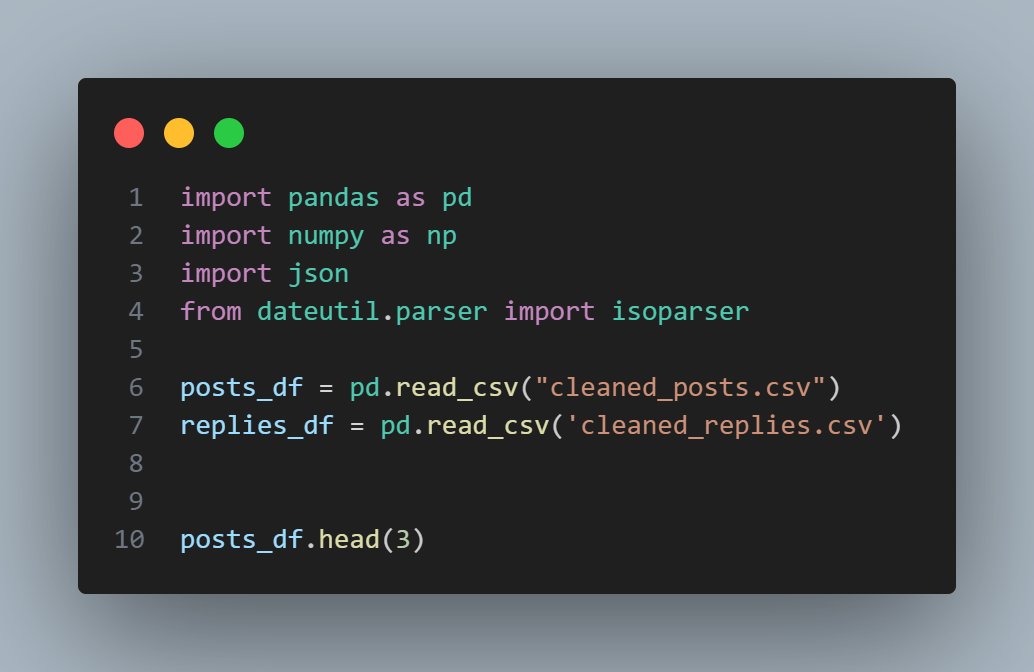
\includegraphics[width=0.5\linewidth]{images/code-3.1.png}
\end{center}

Đây là nơi ta bắt đầu. Ta đọc dữ liệu từ hai tệp CSV: \texttt{cleaned\_posts.csv} và \texttt{cleaned\_replies.csv}.
Các thư viện \texttt{numpy}, \texttt{pandas} cũng được import để hỗ trợ các phép toán số học, xử lý dữ liệu.
Ngoài ra, một số thư viện khác như \texttt{dateutil, json} được khai báo để thực hiện hỗ trợ biến đổi dữ liệu.

\begin{center}
    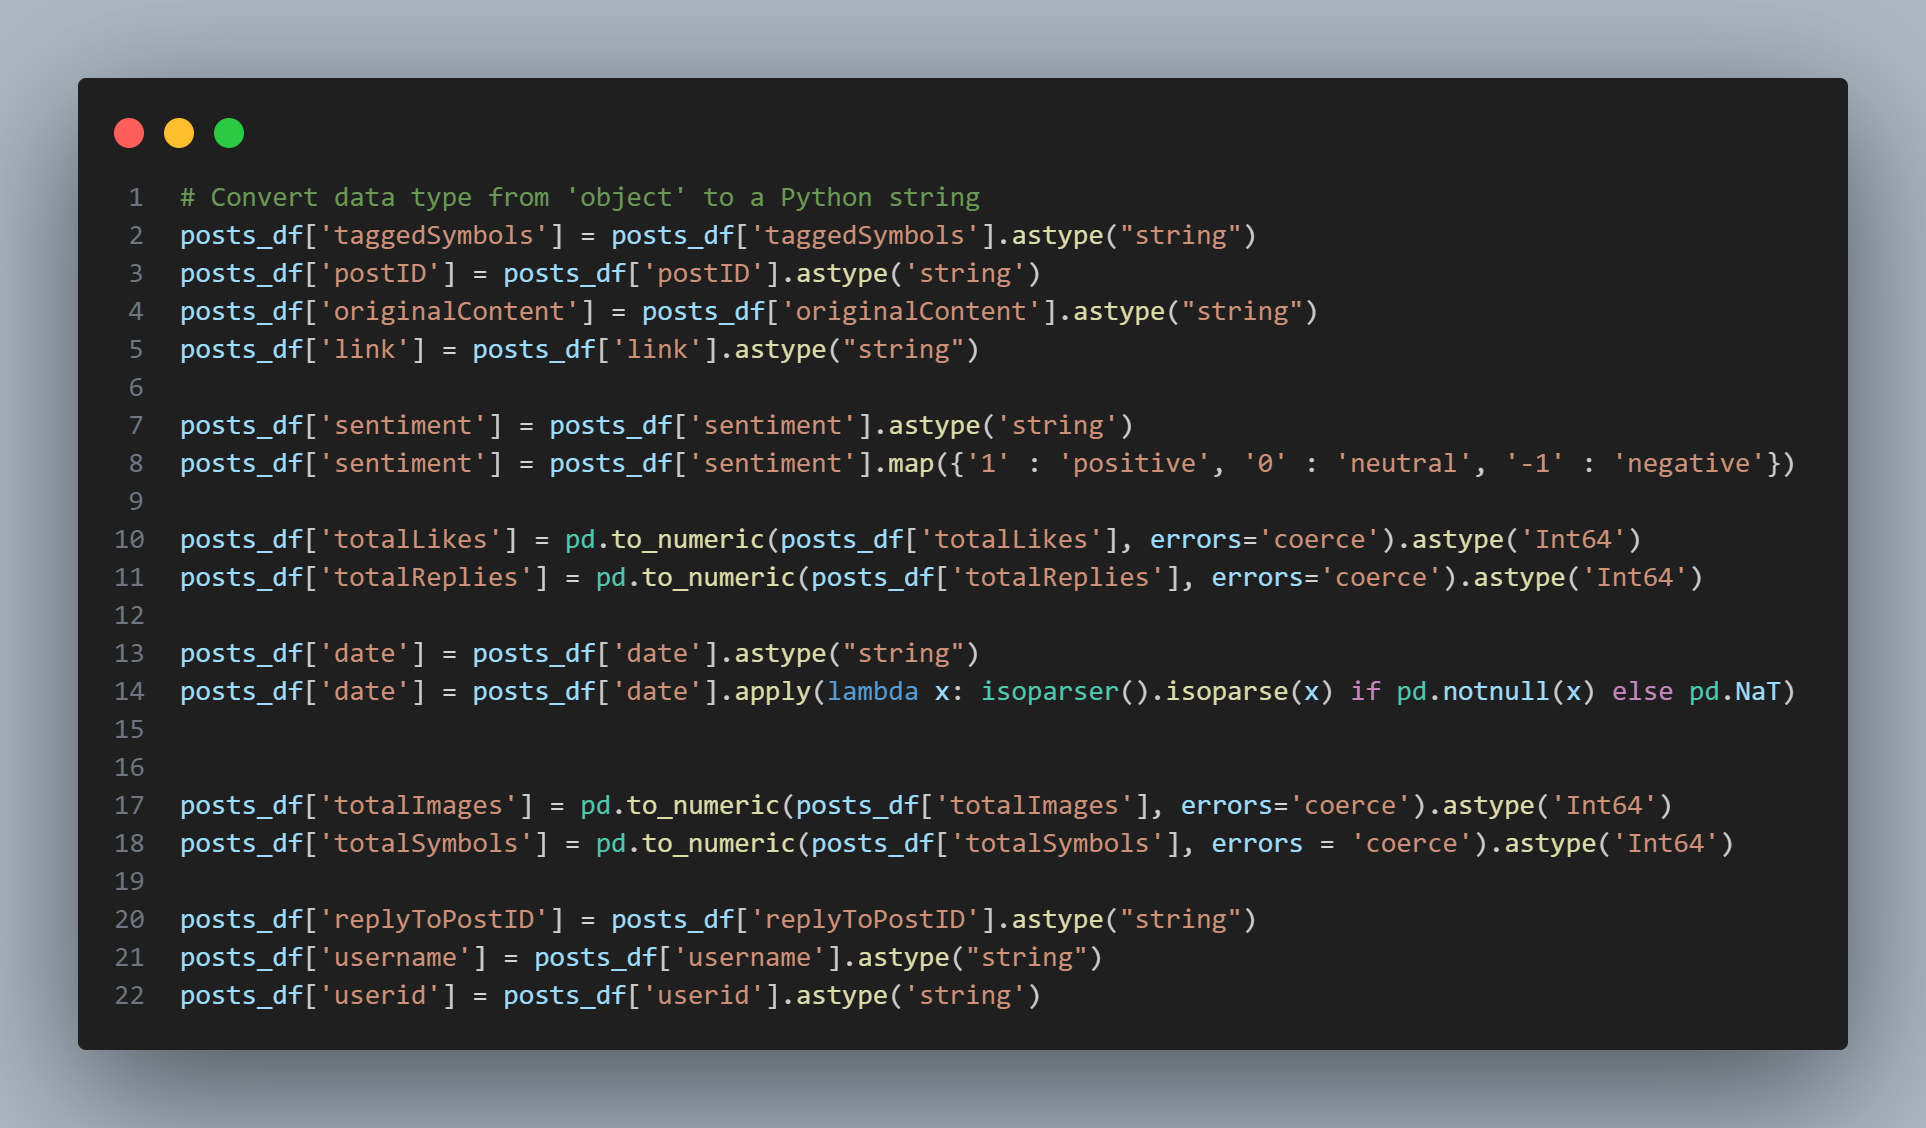
\includegraphics[width=0.9\linewidth]{images/code-3.2.png}
\end{center}

Ta thực hiện chuyển đổi kiểu dữ liệu về các dạng phù hợp cho các cột trong dataframe \texttt{posts\_df}.  
Các bước xử lý bao gồm việc định lại kiểu cột, gán nhãn dữ liệu, dịch thời gian sang dạng DateTime, ...

\subsection*{Xử lý cột \texttt{taggedSymbols}}
Cột \texttt{taggedSymbols} là một cột dữ liệu đặc biệt cần được xử lý riêng. Đây là cột chứa thông tin về các mã chứng khoán và giá của chúng tại thời điểm được nhắc tới. Lưu ý rằng mỗi bài viết có thể đề cập đến nhiều mã chứng khoán cùng một lúc, khiến dữ liệu trong cột này có dạng danh sách, chứa nhiều phần tử.\\

Ta sẽ giải quyết bằng cách sử dụng \texttt{.explode()} trong pandas, hàm này có tác dụng tách một hàng có cột dạng list thành nhiều hàng:
\begin{center}
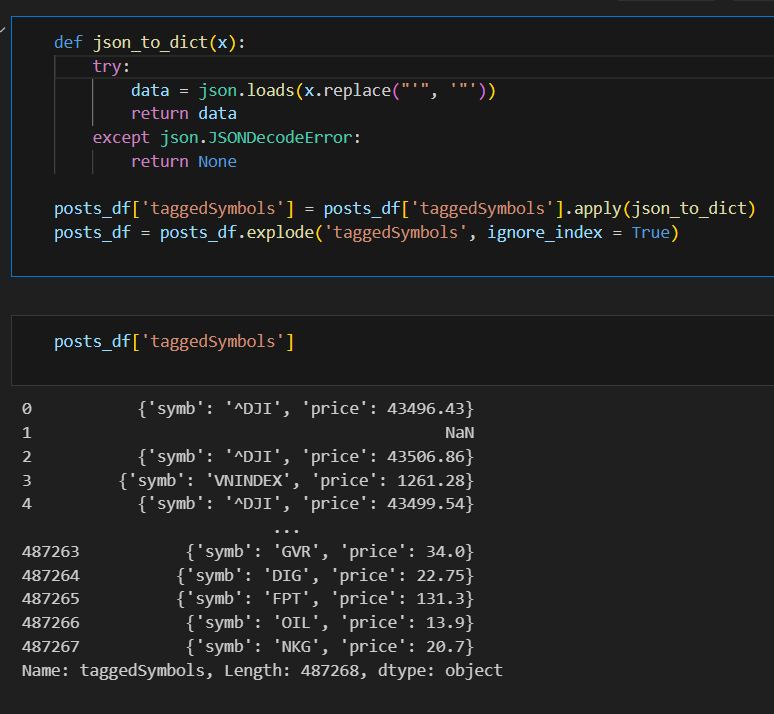
\includegraphics[width=0.7\linewidth]{images/code-3.3.png}
\end{center}

Sau khi tách các mã chứng khoán trong mỗi bài viết thành các hàng riêng biệt, ta thực hiện tách phần này thành hai cột riêng biệt: mã chứng khoán được đề cập (\texttt{symbol}) và giá tại thời điểm đề cập (\texttt{price}). Việc tách này giúp việc theo dõi và phân tích dữ liệu trở nên dễ dàng và trực quan hơn. Dữ liệu các bài viết được lưu trong dataframe \texttt{posts\_df}, dữ liệu bình luận được lưu trong \texttt{replies\_df}.

\begin{center}
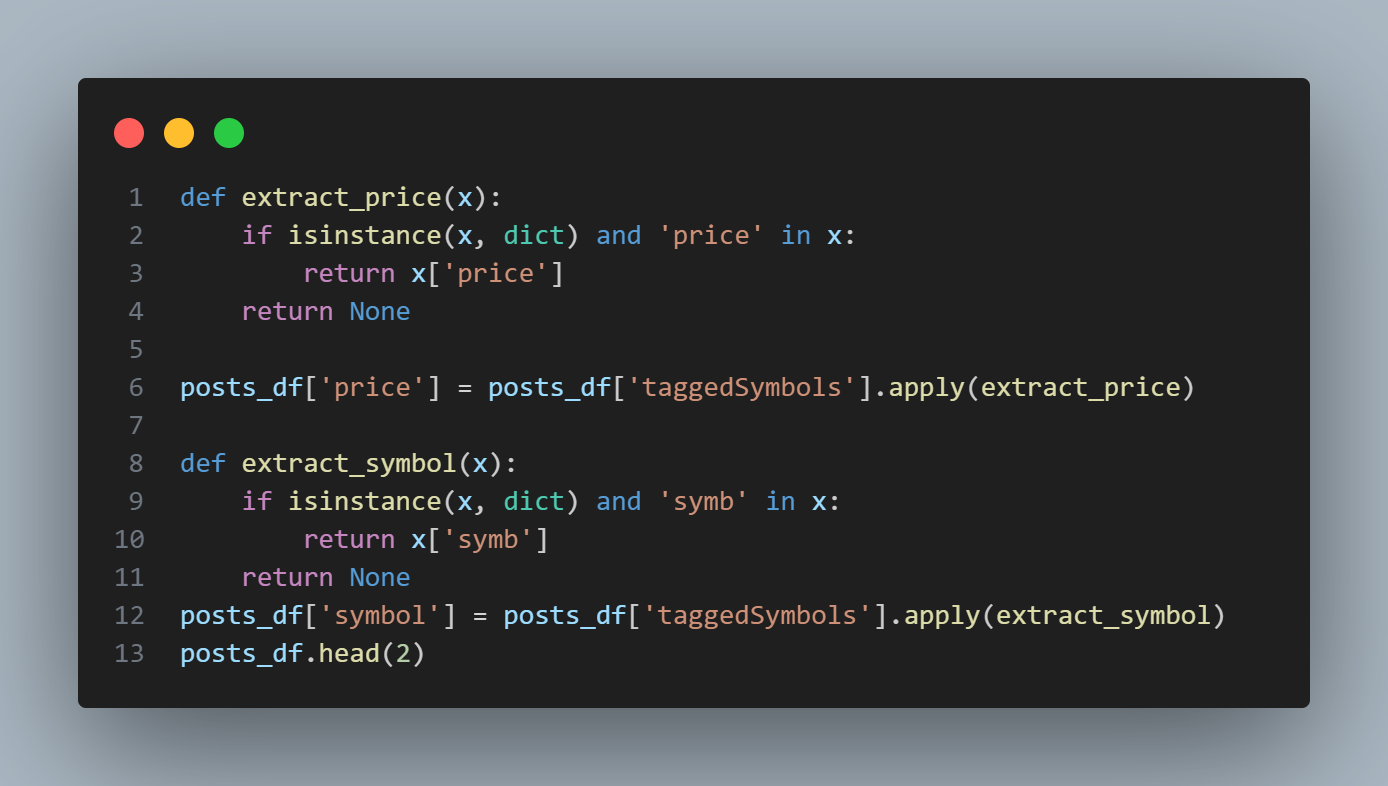
\includegraphics[width=0.75\linewidth]{images/code-3.4.png}
\end{center}

\section{Phân tích dữ liệu bài đăng}

\subsection{Số bài đăng theo ngày}
\begin{figure}[H]
    \centering
    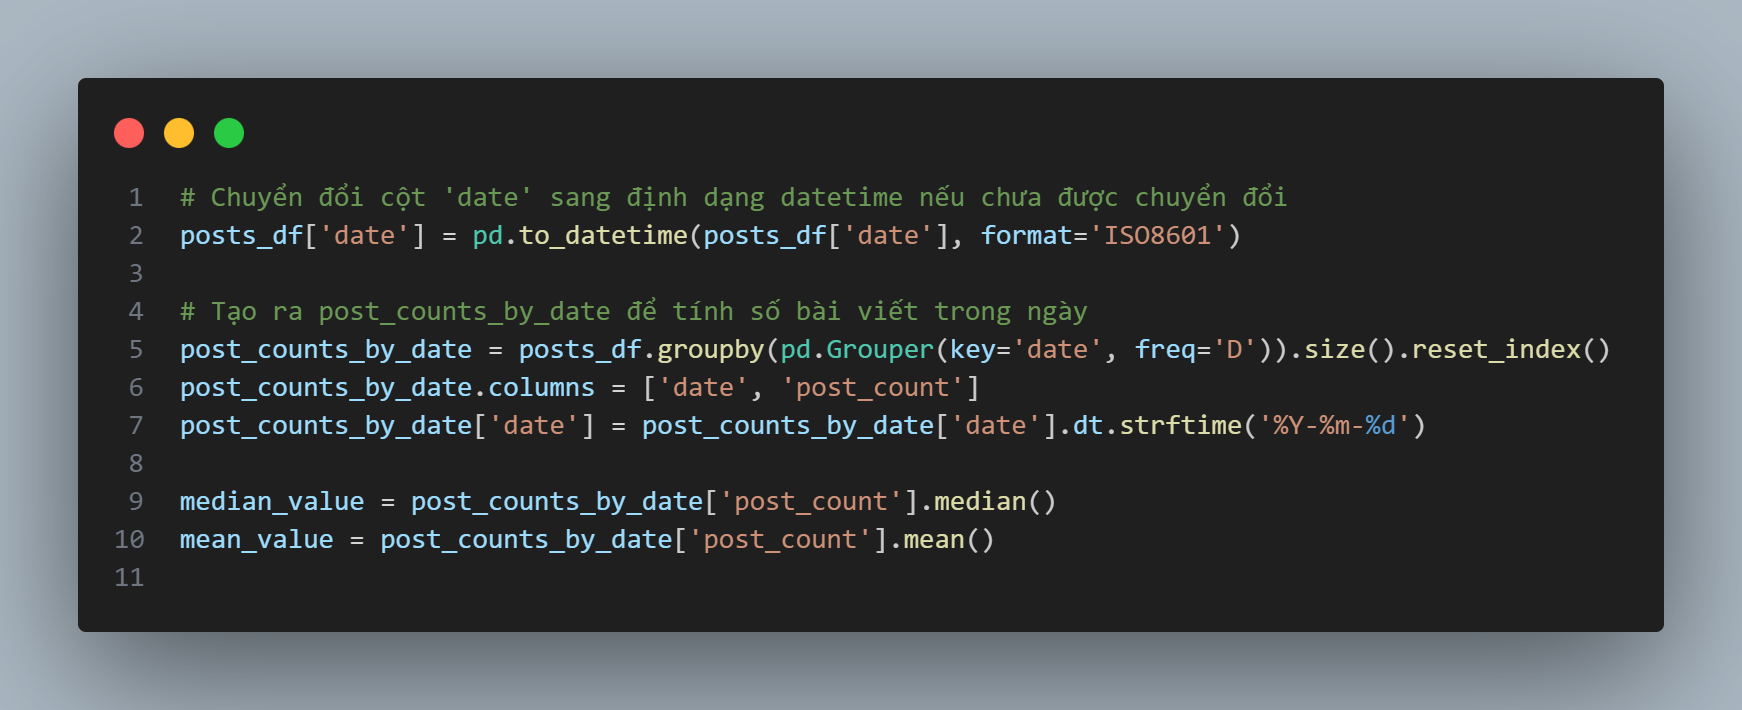
\includegraphics[width=0.75\linewidth]{images/code-2.14.png}
    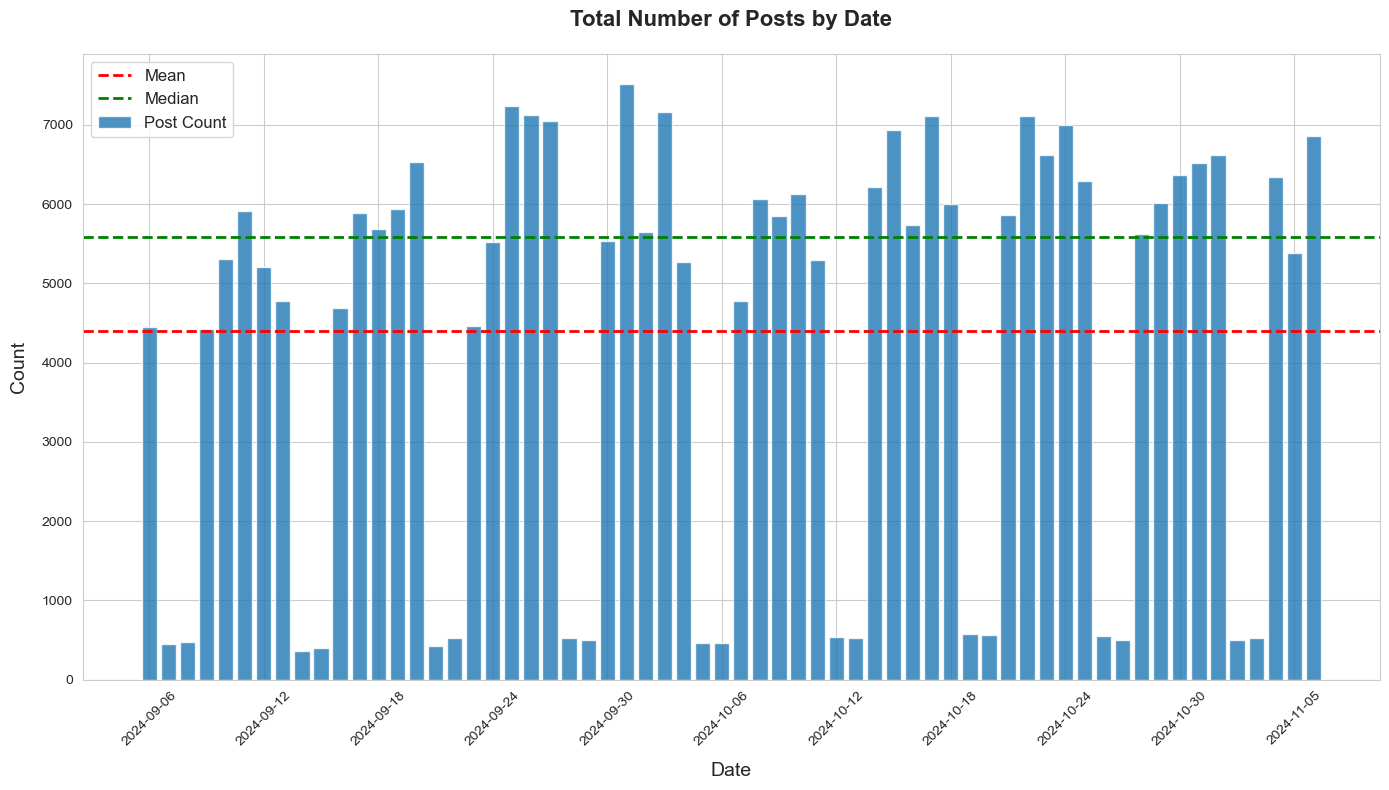
\includegraphics[width=1\linewidth]{images/plot-2.21-column_chart.png}
    \caption{Số lượng bài đăng hàng ngày}
    \label{fig:2.1}
\end{figure}

\textbf{Nhận xét:}
\begin{itemize}
    \item Biểu đồ cho thấy sự chênh lệch đáng kể giữa các ngày. Một số ngày có số bài đăng rất thấp (dưới 1000 bài), trong khi những ngày khác vượt quá 6000 bài, và có chu kì lặp lại.
    \item Những ngày ít bài đăng là những ngày cuối tuần, khi mà thị trường không mở cửa để nhà đầu tư giao dịch. Như vậy sẽ có ít bài viết để nói hơn.
    \item Đường trung bình nằm dưới đường trung vị, cho thấy phân phối có một số ngày có lượng bài đăng rất thấp kéo giá trị trung bình xuống.
    \item Đường trung vị cao hơn đường trung bình, điều này phản ánh rằng phần lớn các ngày có số bài đăng cao hơn giá trị trung bình, nhưng có một vài giá trị ngoại lai thấp (outliers) làm giảm giá trị trung bình.
\end{itemize}

\subsection{Số bài đăng theo ngày trong tuần và giờ}
Có thể thấy diễn đàn có chu kỳ tương tác tương đối thu vị, vậy thì thời gian hoạt động chủ yếu của người dùng là gì?

\begin{figure}[H]
    \centering
    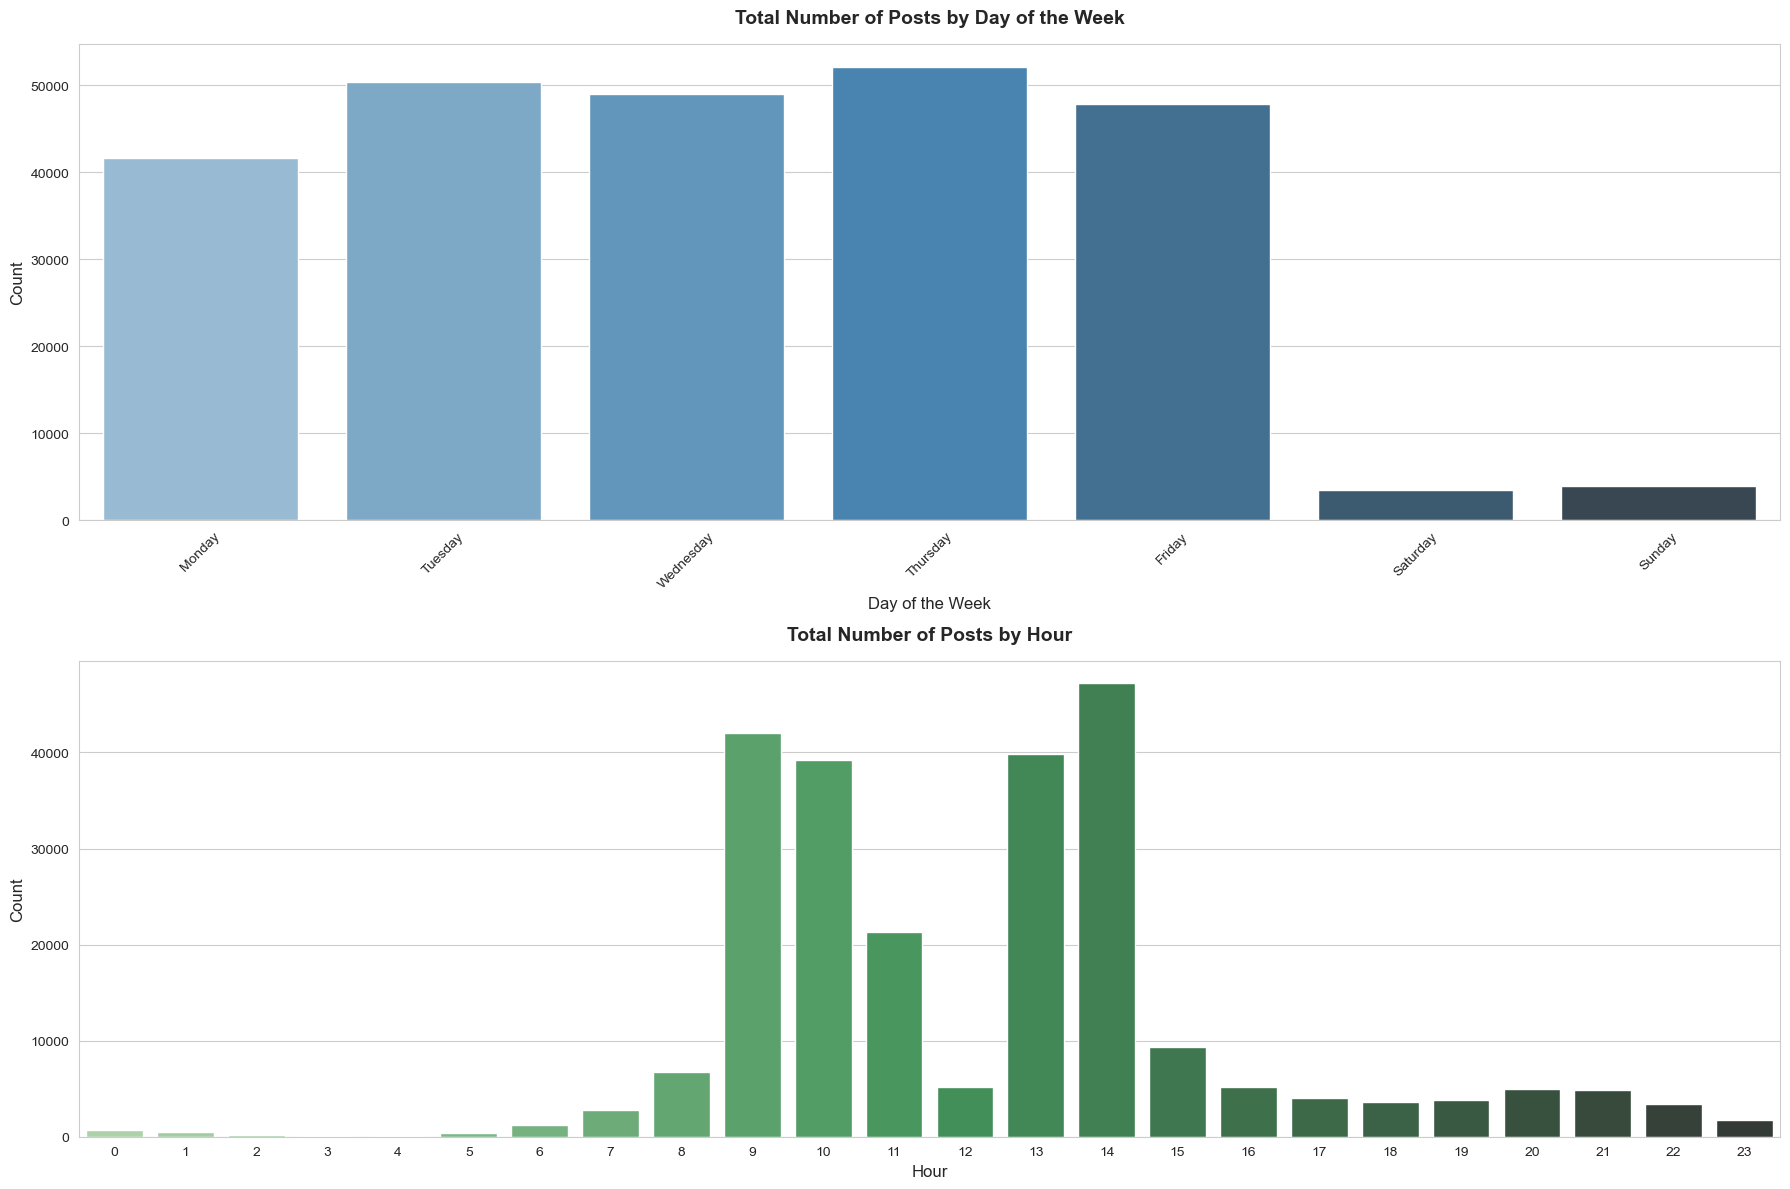
\includegraphics[width=1\linewidth]{images/plot-2.23-column_chart_merge.png}
    \caption{Số lượng bài đăng theo tuần, theo giờ}
    \label{fig:2.2}
\end{figure}
Người dùng hoạt động mạnh nhất vào Thứ 5 và Thứ 3 và hoạt động ít nhất vào các ngày nghỉ là Thứ 7 và Chủ Nhật Khung giờ vàng hay khung giờ cao điểm của người dùng nói chung là từ 9-11h và 13-15h. Tuy nhiên, vào giữa khung giờ vàng, lúc 12h, lượng tương tác đột ngột giảm mạnh, và ngoài các khung giờ này, mức độ tương tác cũng rất thấp. \\

Lý do là bởi thị trường chứng khoán Việt Nam hoạt động từ Thứ 2 - Thứ 6, mở cửa vào lúc 9h-11h30, nghỉ trưa từ 11h30-13h, sau đó mở cửa từ lúc 13h-15h. Ta dễ dàng thấy khung giờ mà số lượng bài viết nhiều nhất trùng khớp với khoảng thời gian này.

\subsection{Phân bố Quan điểm người dùng}
\begin{wrapfigure}[16]{H}{0.3\textwidth}
\raggedright
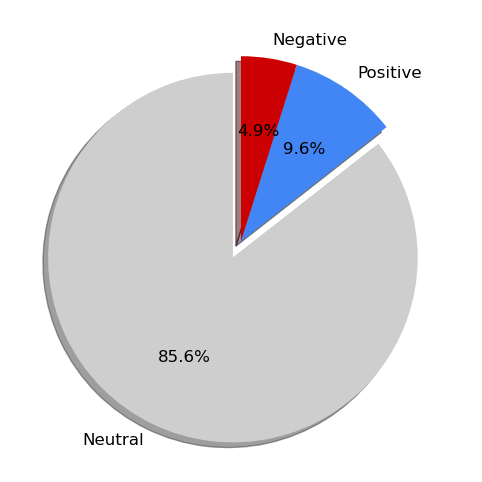
\includegraphics[width=.98\linewidth]{images/plot-2.27-senanalysis.png}

\caption{Phân bố Quan điểm người dùng}
\label{fig:2.30}
\end{wrapfigure}

Theo hình (\ref{fig:2.30}), hầu hết (85.6\%) bài đăng đều mang quan điểm Trung lập. Điều này phần lớn là do thói quen không đặt quan điểm cho bài viết của người dùng. Ngoài ra, số lượng bài Tích cực (9.6\%) lớn gần gấp đôi so với Tiêu cực (4.9\%), cho thấy xu hướng chung của diễn đàn là tương đối tích cực, ít nhất là trong khoảng dữ liệu hai tháng.

\subsection{Wordcloud bài đăng}

Về nội dung bài viết, ta có thể tìm ra những từ khóa nào được người dùng sử dụng nhiều. Bằng cách sử dụng word cloud ta có mô phỏng như sau (hình (\ref{fig:2.3})):\\

Như vậy có thể thấy, ngoài \textbf{cổ phiếu}, \textbf{giao dịch}, \textbf{thị trường} thì có một số keyword đáng chú ý khác là \textbf{thanh khoản}, \textbf{điểm mua,} \textbf{kỳ vọng }là những keyword đáng chú ý. Có thể thấy diễn đàn có xu hướng khá tích cực, khi sử dụng nhiều từ như \textbf{hỗ trợ, tăng trưởng, tích lũy, tiếp tục, xu hướng,} ...

\begin{figure}[H]
    \centering
    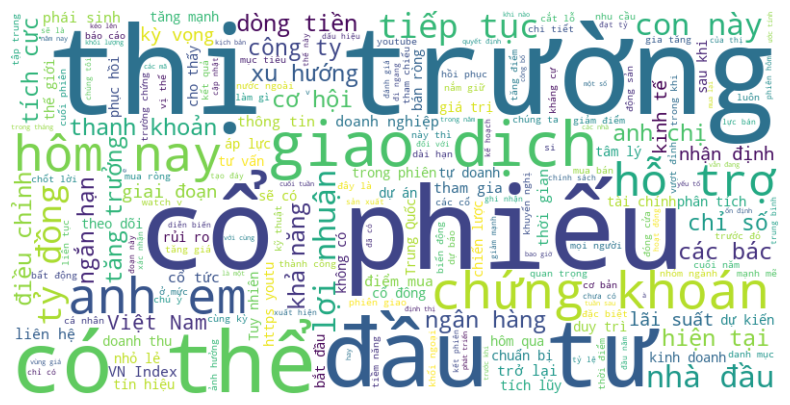
\includegraphics[width=0.9\linewidth]{images/plot-2.1-wordcloud.png}
    \vspace{-1em}
    \caption{Wordcloud bài viết}
    \label{fig:2.3}
\end{figure}

\subsubsection{Biểu diễn keyword dựa trên quan điểm của người dùng}

Trong dữ liệu của mỗi bài viết có mục về quan điểm (sentiment) của người dùng trong bài viết đó, vì vậy ta có thể sử dụng chúng để chia thành hai word cloud theo quan điểm của từng người như sau:

\begin{figure}[H]
  \begin{subfigure}{.5\textwidth}
  \centering
    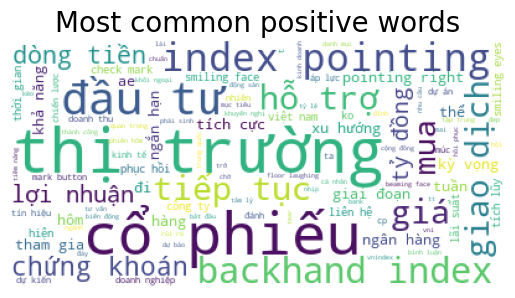
\includegraphics[width=1\linewidth]{images/plot-2.15-wordcloud.png}
  \end{subfigure}%
  \begin{subfigure}{.5\textwidth}
  \centering
    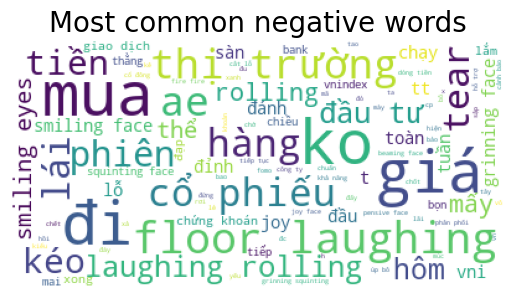
\includegraphics[width=1\linewidth]{images/plot-2.16-wordcloud.png}
  \end{subfigure}
  \vspace{-2em}
  \caption{Một số từ hàm ý Tích cực và Tiêu cực xuất hiện nhiều nhất}
  \label{fig:2.4}
\end{figure}

\textbf{Nhận xét:}
\begin{itemize}
\item Giữa 2 wordcloud ta có thể thấy có một số keyword trùng lặp như \textbf{cổ phiếu, giá, thị trường, đầu tư}.
\item Các bài tiêu cực, lại không có nhiều từ mang hàm ý tiêu cực. Trong khi các bài tích cực thì vẫn theo xu hướng chung của diễn đàn.
\item Trong các bài thường có xu hướng xuất hiện nhiều từ như \textbf{index pointing, backhand index, laughing rolling, ...} là các emoji. Điều này cho thấy mức độ sử dụng emoji trong các bài viết là tương đối lớn.
\end{itemize}

\subsection{Số lần xuất hiện của link}
\begin{center}
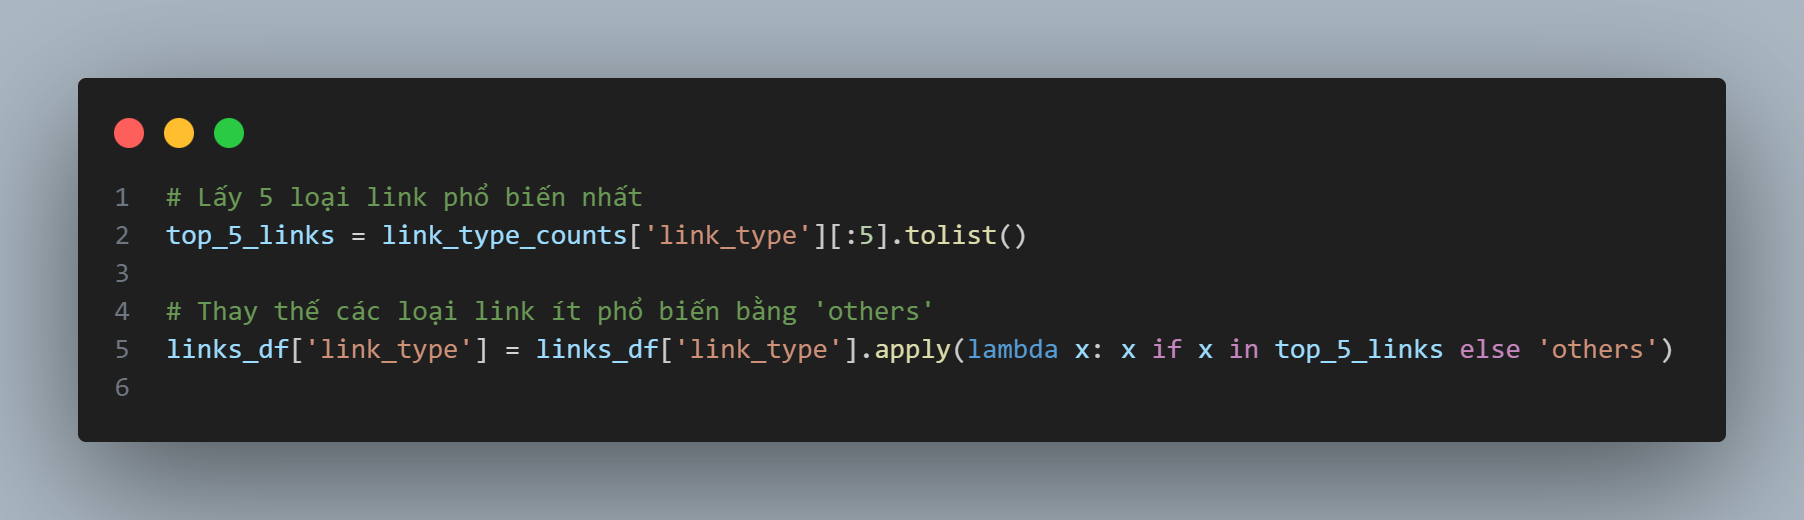
\includegraphics[width=0.75\linewidth]{images/code-2.16.png}
\end{center}

\begin{figure}[H]
    \centering
    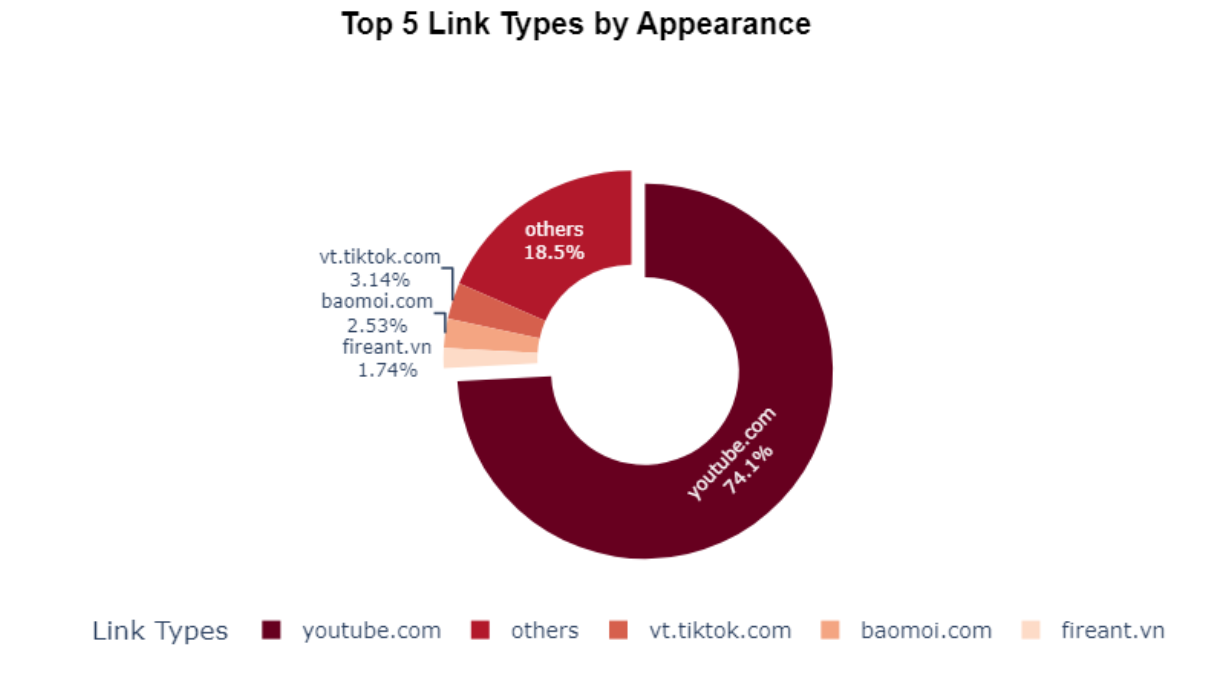
\includegraphics[width=0.9\linewidth]{images/plot-2.2-doughnut_chart.png}
    \caption{Top 5 loại link xuất hiện nhiều nhất}
    \label{fig:2.5}
\end{figure}

\textbf{Nhận xét:}
\begin{itemize}
    \item Có thể thấy rằng đa số các liên kết trong bài viết đều dẫn đến các trang web bên ngoài, trong đó có nhiều liên kết đến \textbf{youtube.com}. 
    \item Giải thích cho điều này là vì YouTube là nền tảng cho phép upload video và là nền tảng livestream với số lượng người theo dõi rất đông đảo, đồng thời cho phép kiếm tiền vậy nên các video thường có xu hướng cập nhật thông tin rất nhạy so với thị trường.
    \item Người dùng thường hay lấy những thông tin được dẫn chứng từ các video YouTube, cũng như các chuyên gia hay chia sẻ nhận định hoặc livestream trên nền tảng này.
    \item Các trang còn lại có sự phân bố tỉ lệ khá đều và nhỏ lẻ với $3.14\%$ từ \textbf{tiktok.com}, $2.53\%$ từ \textbf{baomoi.com} và $1.74\%$ từ \textbf{fireant.vn}.
    \item Còn lại là các mã có tỉ lệ xuất hiện ít hơn tổng hợp lại trong \textbf{Others} với $18.5\%$.
\end{itemize}
            
\subsection{Quan điểm người dùng khi chèn đường link}

\begin{center}
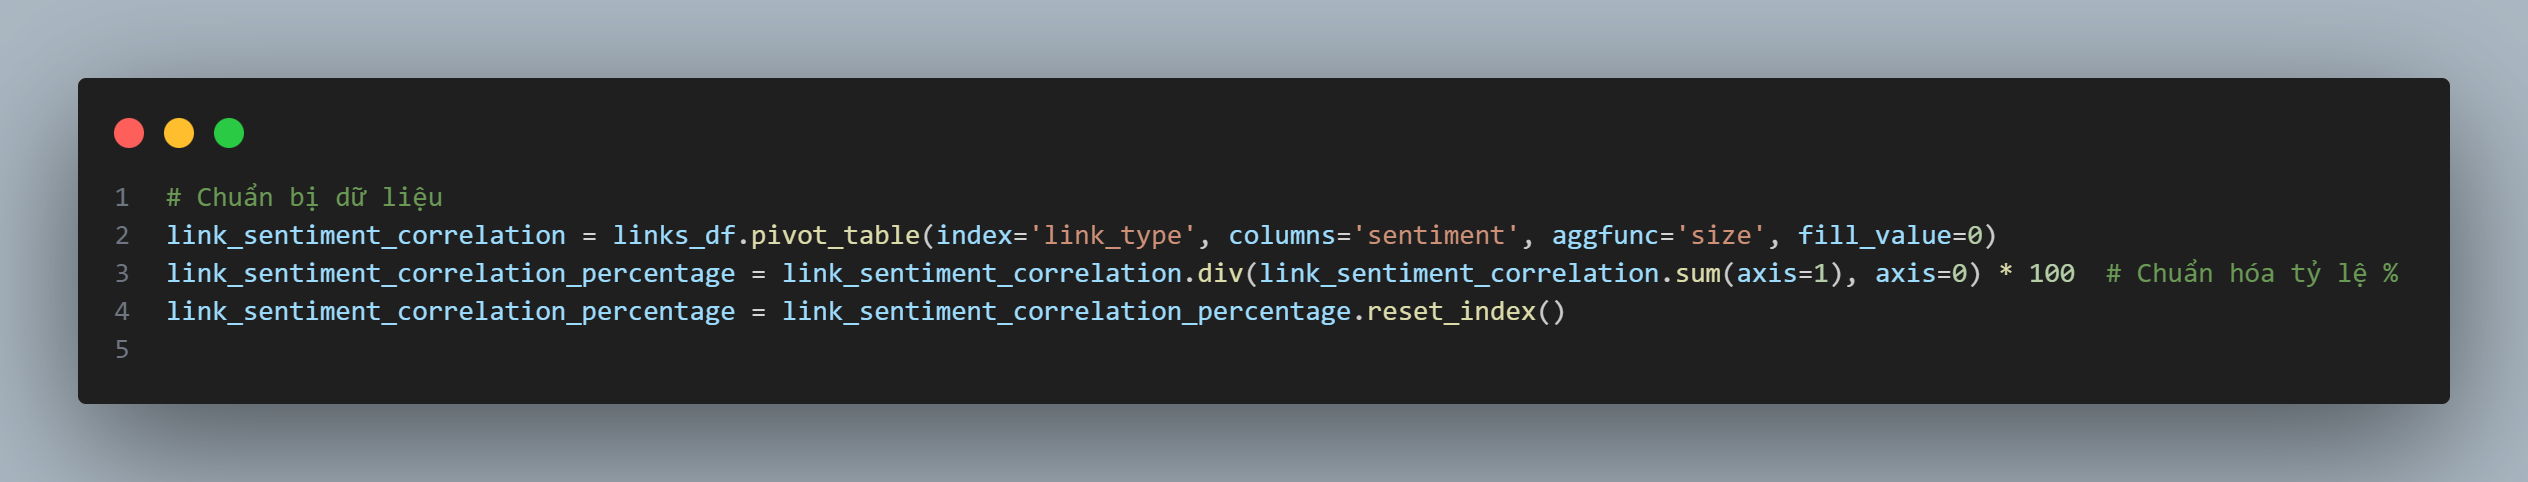
\includegraphics[width=0.9\linewidth]{images/code-2.17.png}
\end{center}

Đặt câu hỏi về phản ứng của người đăng bài khi họ nhắc đến các đường đẫn như nào. Để biểu diễn kĩ hơn, ta sử dụng heatmap để miêu tả sự phân bố của các sentiment (hình (\ref{fig:2.6})). Từ biểu đồ heatmap (\ref{fig:2.6}), ta có thể rút ra một số nhận xét:

\begin{itemize}
    \item \textbf{youtube.com}: Nền tảng chia sẻ video, đây là loại liên kết phổ biến nhất và có sự phân bố lệch hẳn về phía Trung lập. 
    \item \textbf{vt.tiktok.com}: Nền tảng chia sẻ video ngắn, loại liên kết này chủ yếu có quan điểm trung lập và tích cực, với số lượng quan điểm trung lập chiếm phần lớn.
    \item \textbf{fireant.vn}: Liên kết trong FireAnt, loại liên kết này chủ yếu có sentiment trung lập, với số lượng quan điểm tiêu cực và tích cực ít hơn.
    \item \textbf{baomoi.com}: Trang báo tổng hợp thông tin, số lượng liên kết từ baomoi.com có quan điểm tiêu cực và tích cực gần như tương đương, trong khi sentiment trung lập ít hơn.
    \item Những liên kết khác: Các liên kết khác ngoài top 4 chủ yếu có quan điểm trung lập, nhưng cũng có một số lượng đáng kể quan điểm tích cực và tiêu cực.

\end{itemize}

\begin{figure}[h]
    \centering
    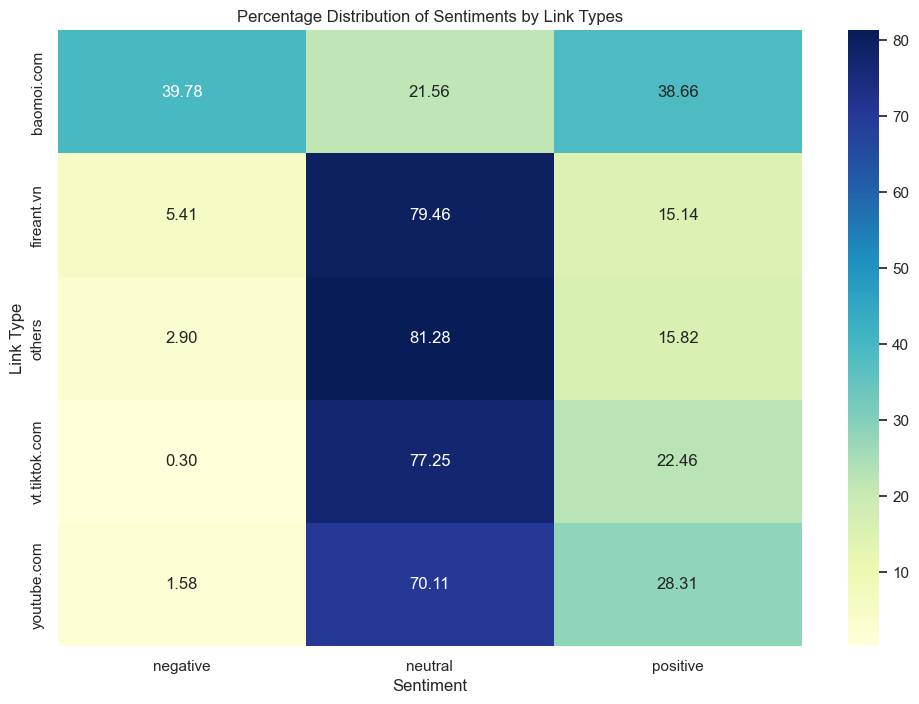
\includegraphics[width=0.85\linewidth]{images/plot-2.4-heatmap.png}
    \caption{Heatmap tỉ lệ phản ứng người dùng với liên kết}
    \label{fig:2.6}
\end{figure}

Các bài viết khi kèm link phần lớn là Tích cực hoặc Trung lập. Tuy nhiên các liên kết từ \textbf{baomoi.com} có sự phân bố quan điểm đa dạng hơn. Lý do có thể tới từ việc \textbf{baomoi.com} là một trang báo tổng hợp thông tin, nhiều thông tin kiểm chứng từ báo đài được đưa ra, củng cố cho luận điểm đa dạng của người dùng.

\section{Phân tích phản hồi/bình luận}
Ta có cấu trúc dataframe \texttt{replies\_df} giống với \texttt{posts\_df}, do bình luận được lưu trong Cơ sở dữ liệu của FireAnt như một loại bài viết đặc biệt. Vì vậy ta không phải viết lại nhiều code.

\subsection{Số phản hồi theo ngày}
Ta miêu tả số lượng phản hồi theo ngày dưới dạng chart với code sau:

\begin{center}
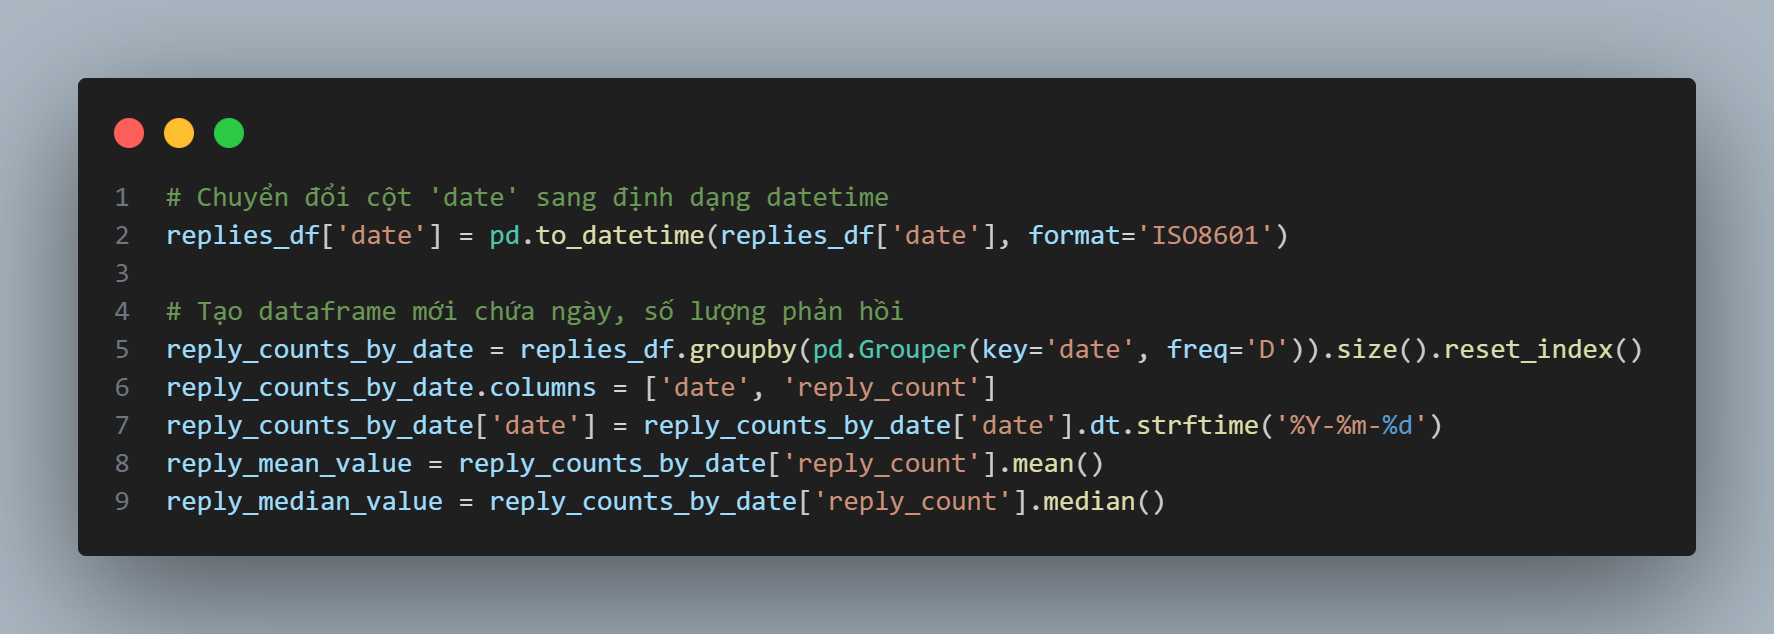
\includegraphics[width=0.8\linewidth]{images/code-2.18.png}
\end{center}

\begin{figure}[H]
    \centering
    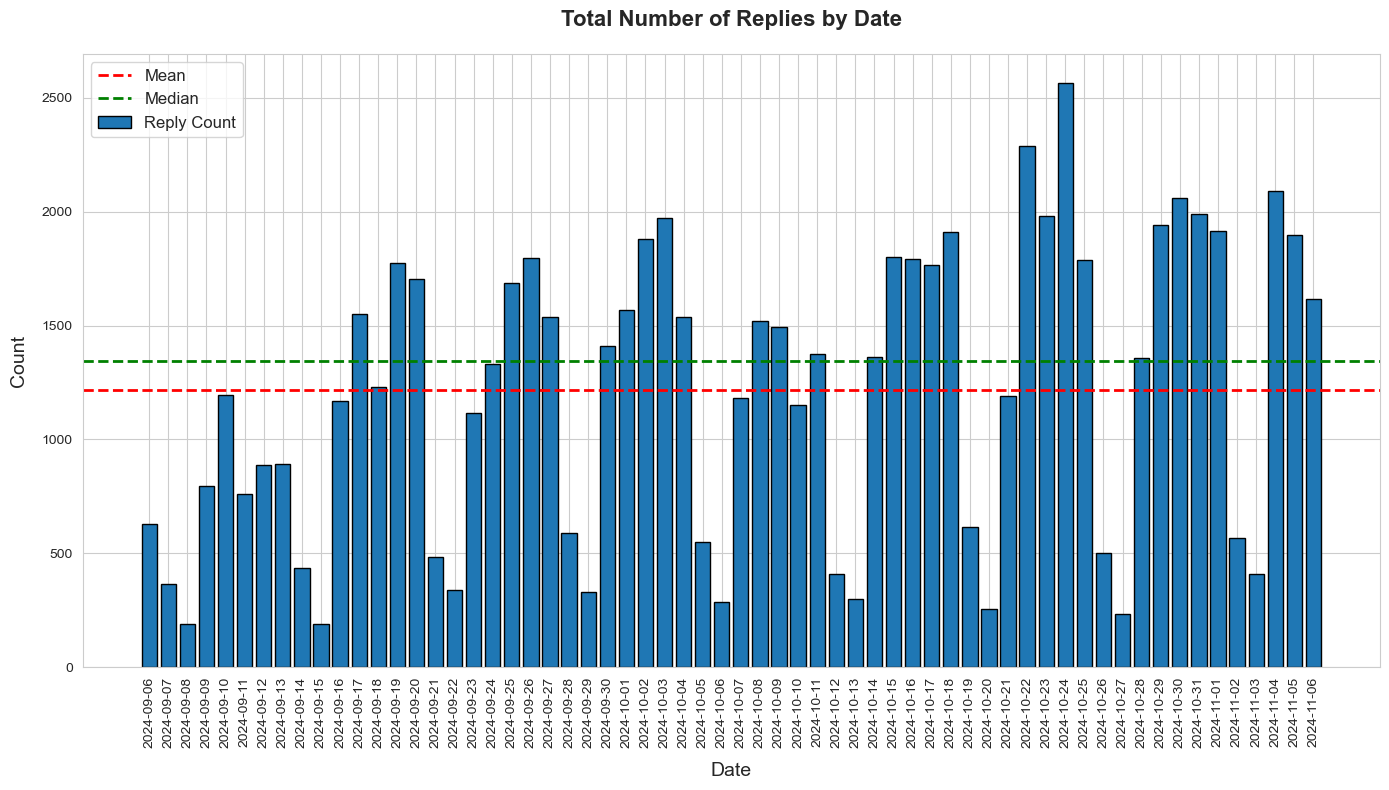
\includegraphics[width=1\linewidth]{images/plot-2.22-column_chart.png}
    \caption{Số lượng các phản hồi theo ngày}
    \label{fig:2.8}
\end{figure}

\textbf{Nhận xét:}

\begin{itemize}
    \item Nhìn chung, số lượng liên kết dao động trong khoảng từ dưới 50 đến hơn 250, với một số ngày có số lượng rất thấp.
    \item Số lượng bình luận có sự tương quan rất lớn với số lượng bài viết, khi cũng có cùng một ``chu kỳ'' với lượng bài viết, là nhiều vào những ngày trong tuần, và ít đi ở những ngày cuối tuần.
    \item Giá trị trung bình thấp hơn giá trị trung vị, cho thấy có những ngày số lượng liên kết rất thấp làm giảm giá trị trung bình. Đường trung vị cao hơn đường trung bình, cho thấy rằng phần lớn các ngày có số lượng liên kết lớn hơn giá trị trung bình, nhưng có một vài ngày với số lượng liên kết rất thấp (outliers).
\end{itemize}

\subsection{Số phản hồi theo ngày trong tuần và giờ}

\begin{center}
    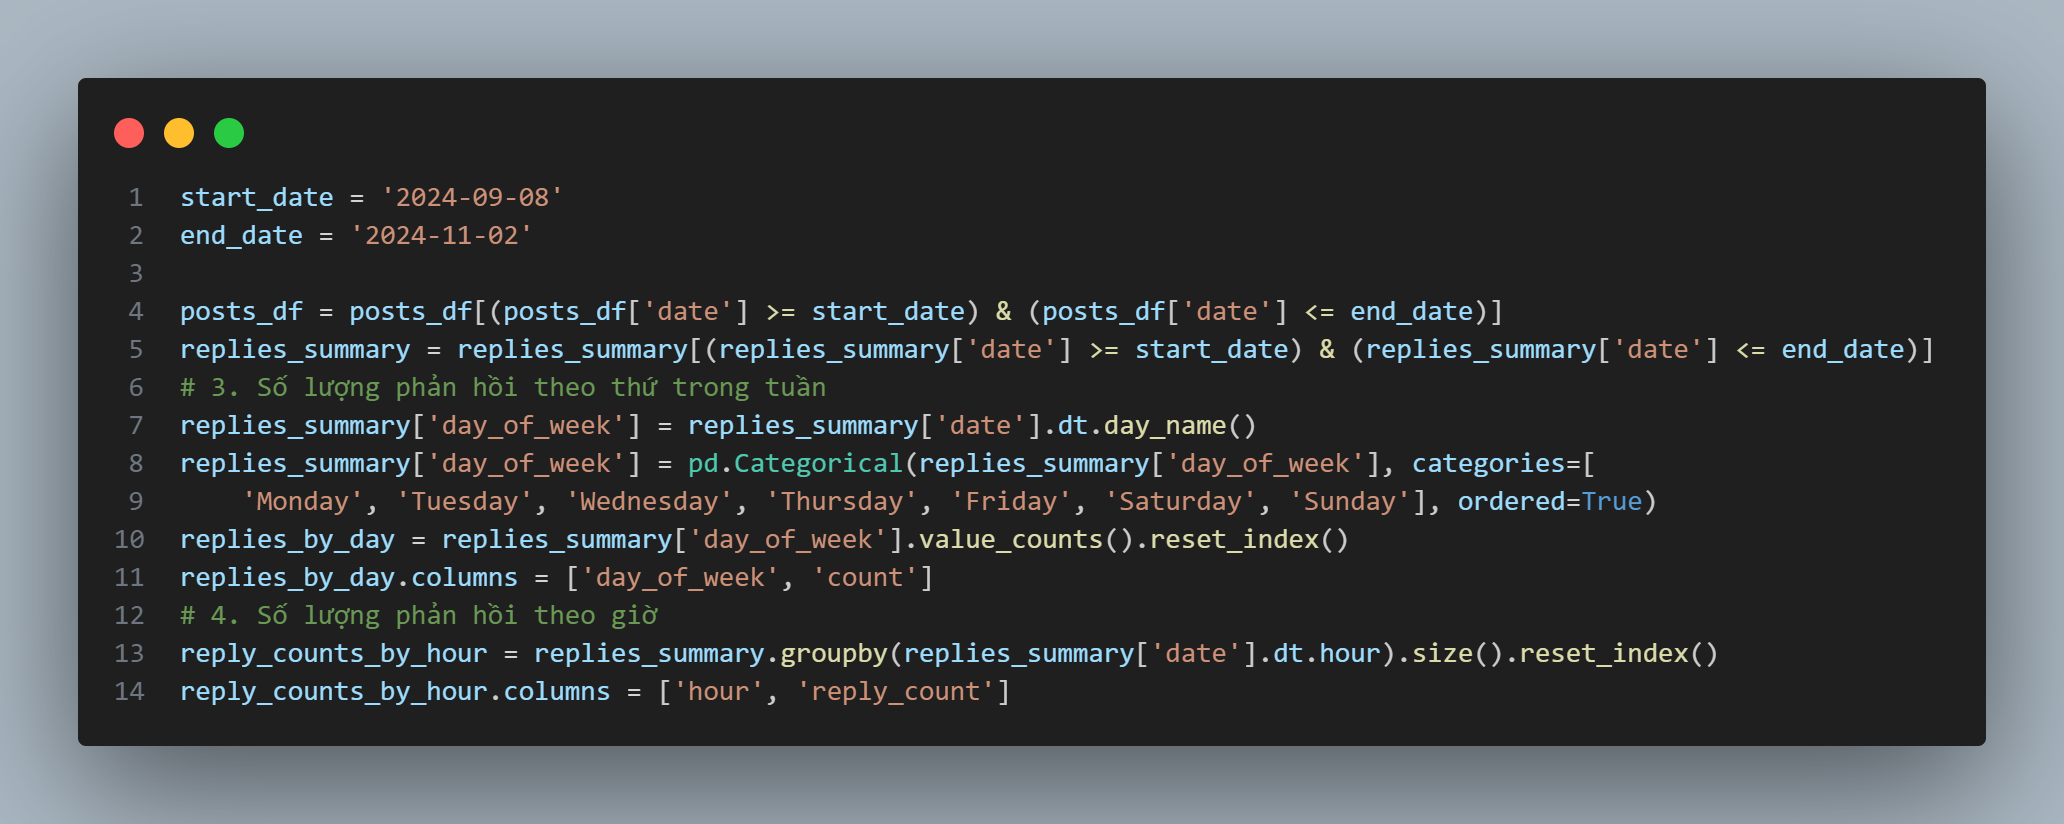
\includegraphics[width=1\linewidth]{images/code-2.23.png}
\end{center}

Như phần trên đã phân tích, dù đồ thị của lượt phản hồi theo tuần và theo giờ có sự tương đồng lớn với đồ thị của số lượng bài viết, nhưng cũng có vài điểm khá nổi bật.

\begin{figure}[H]
    \centering
    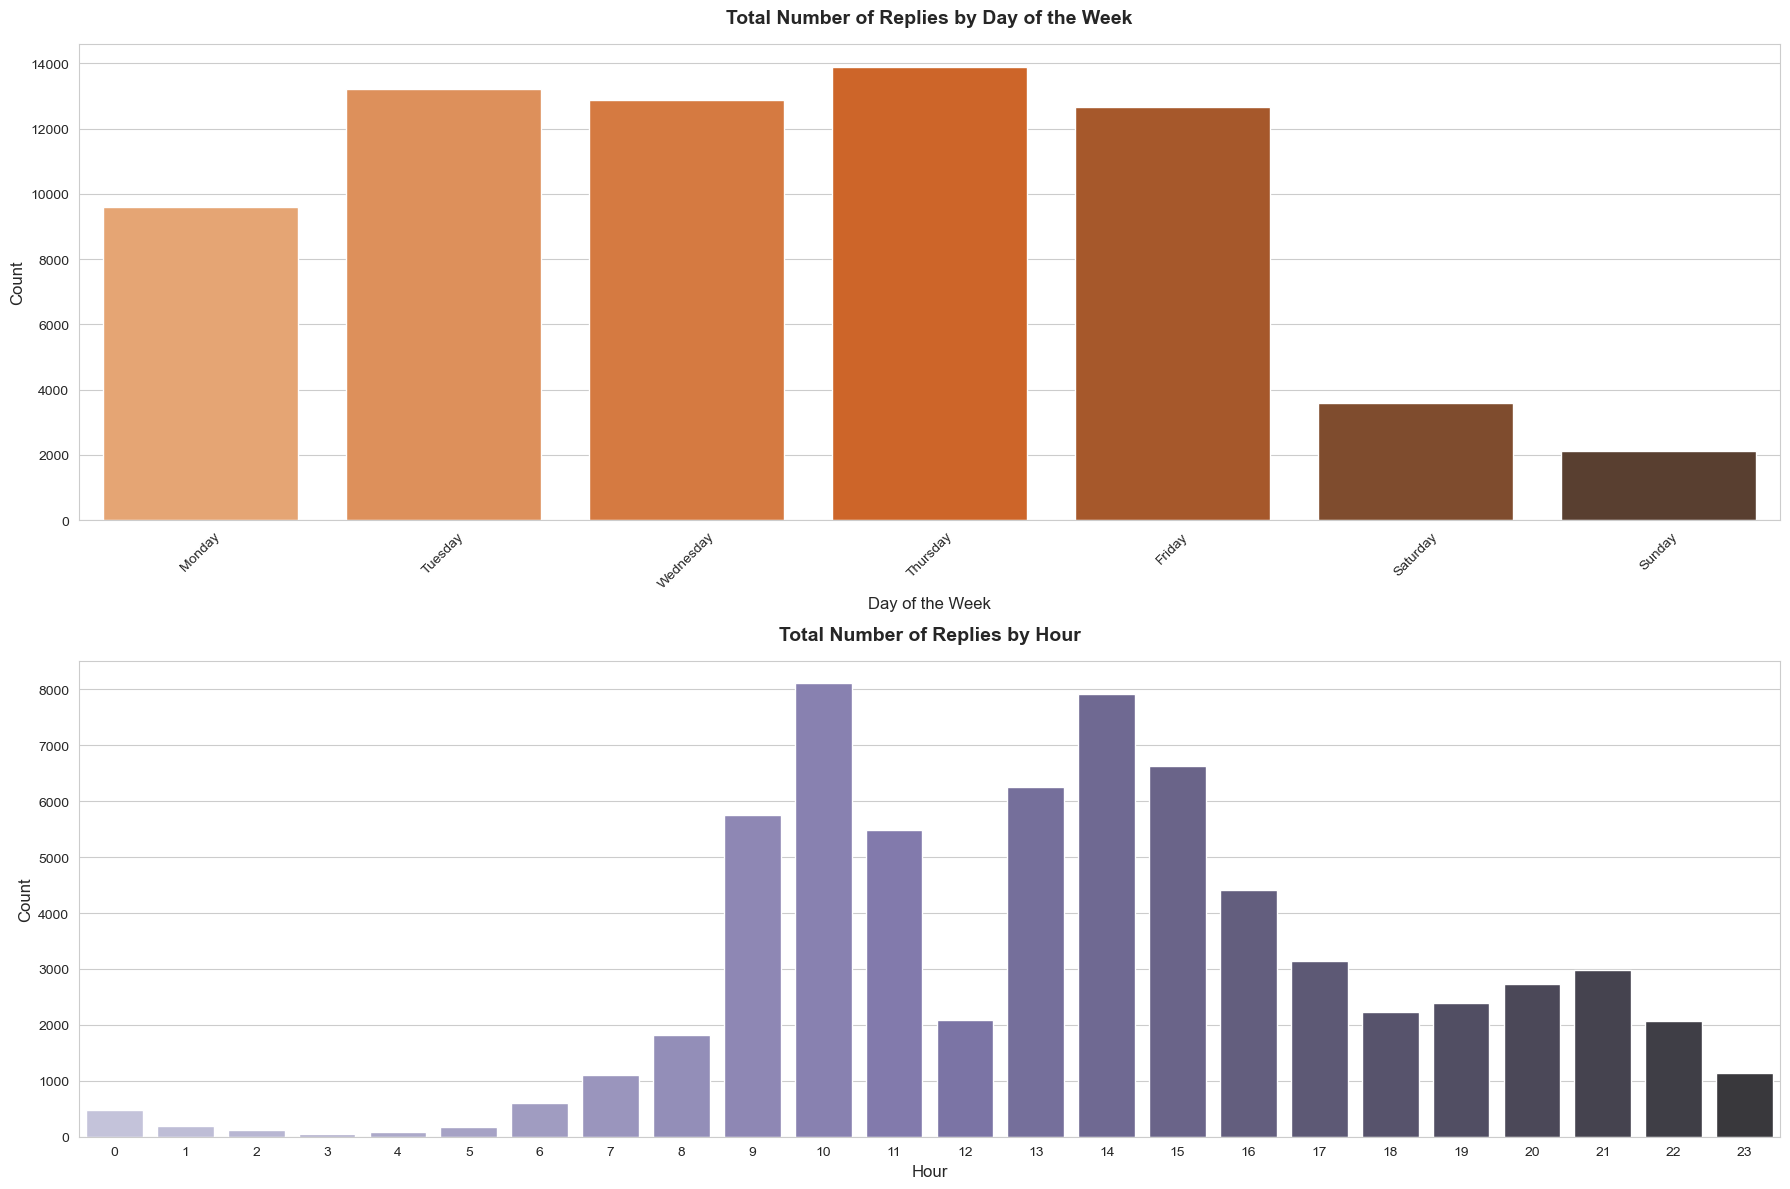
\includegraphics[width=1\linewidth]{images/plot-2.24-column_chart_merge.png}
    \caption{Số lượng phản hồi theo ngày trong tuần và giờ}
    \label{fig:2.9}
\end{figure}
\textbf{Nhận xét:}

\begin{itemize}
    \item Người dùng hoạt động mạnh nhất vào Thứ 5 và Thứ 3 và hoạt động ít nhất vào các ngày nghỉ là Thứ 7 và Chủ Nhật. Khung giờ vàng hay khung giờ cao điểm của người dùng là 9-12h và 13-15h và giữa khung giờ vàng là 12h đột ngột giảm, tương tự như đồ thị của bài viết.
    \item Đặc biệt, khác với đồ thị của nọi dung bài viết, khoảng thời gian từ 15h đổ đi có sự giảm đều, nhẹ và tăng nhẹ lên và đạt đỉnh vào 21h rồi giảm. Có nhiều lý do, thứ nhất, khung thời gian từ 19h-22h là khoảng thời gian nghỉ tối, sẽ có nhiều người có khả năng trực tuyến hơn. Thứ hai, thời điểm 21h là thời điểm sàn chứng khoán Mỹ NASDAQ, NYSE hoạt động, vì vậy nhiều thông tin ở đó được đem ra bàn luận hơn.
\end{itemize}

\subsection{Wordcloud phản hồi}
Tương tự như phần trên, với wordcloud, ta biểu diễn các keyword mà người dùng nói đến trong phần nội dung của bình luận. 

\begin{figure}[H]
    \centering
    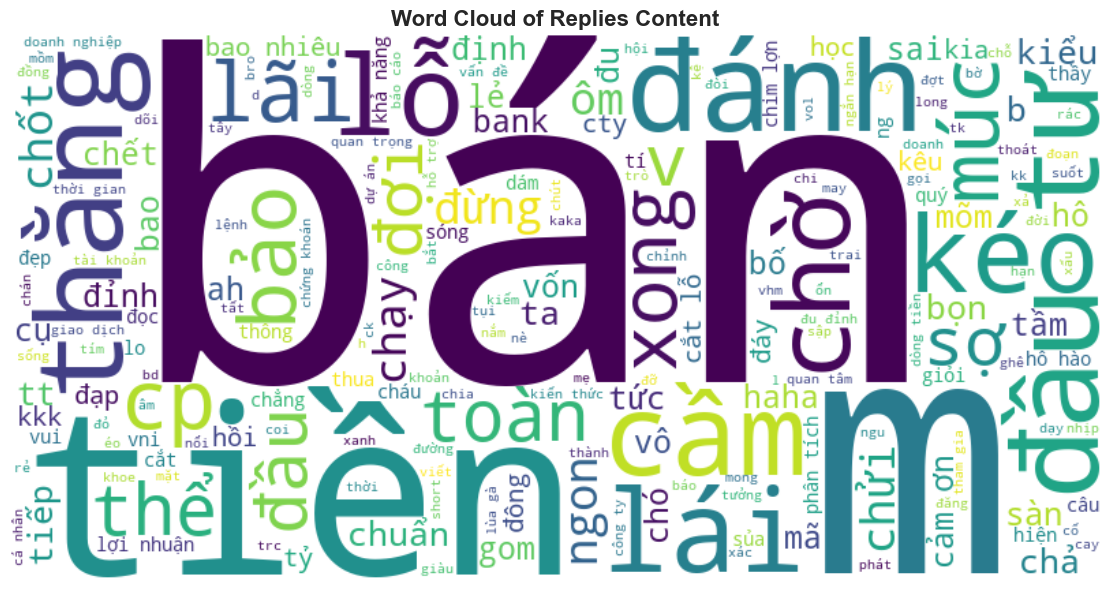
\includegraphics[width=0.5\linewidth]{images/plot-2.12-wordcloud.png}
    \caption{Wordcloud phản hồi (sau khi lọc stopword)}
    \label{fig:2.10}
\end{figure}
Các keyword không có giá trị sử dụng quá nhiều, thường là các từ được sử dụng trong giao tiếp, cũng như liên quan đến chứng khoán.

\section{Phân tích các mã cổ phiếu được đề cập}

\subsection{Quan điểm của người dùng}
Lập một biểu đồ biểu diễn gồm 50 mã có số lần đề cập đến nhiều nhất, tương ứng là số quan điểm của người dùng khi nhắc đến cổ phiếu đó:

\begin{center}
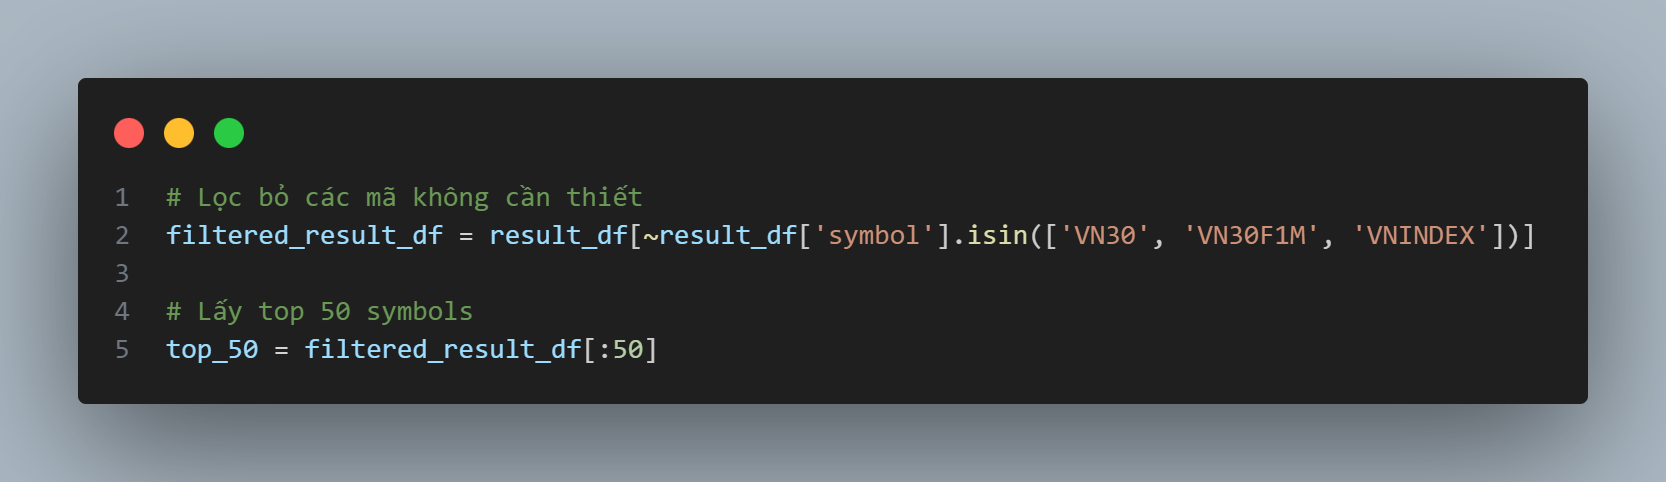
\includegraphics[width=0.8\linewidth]{images/code-2.19.png}
\end{center}
\vspace{-0.5em}
\begin{figure}[H]
    \centering
    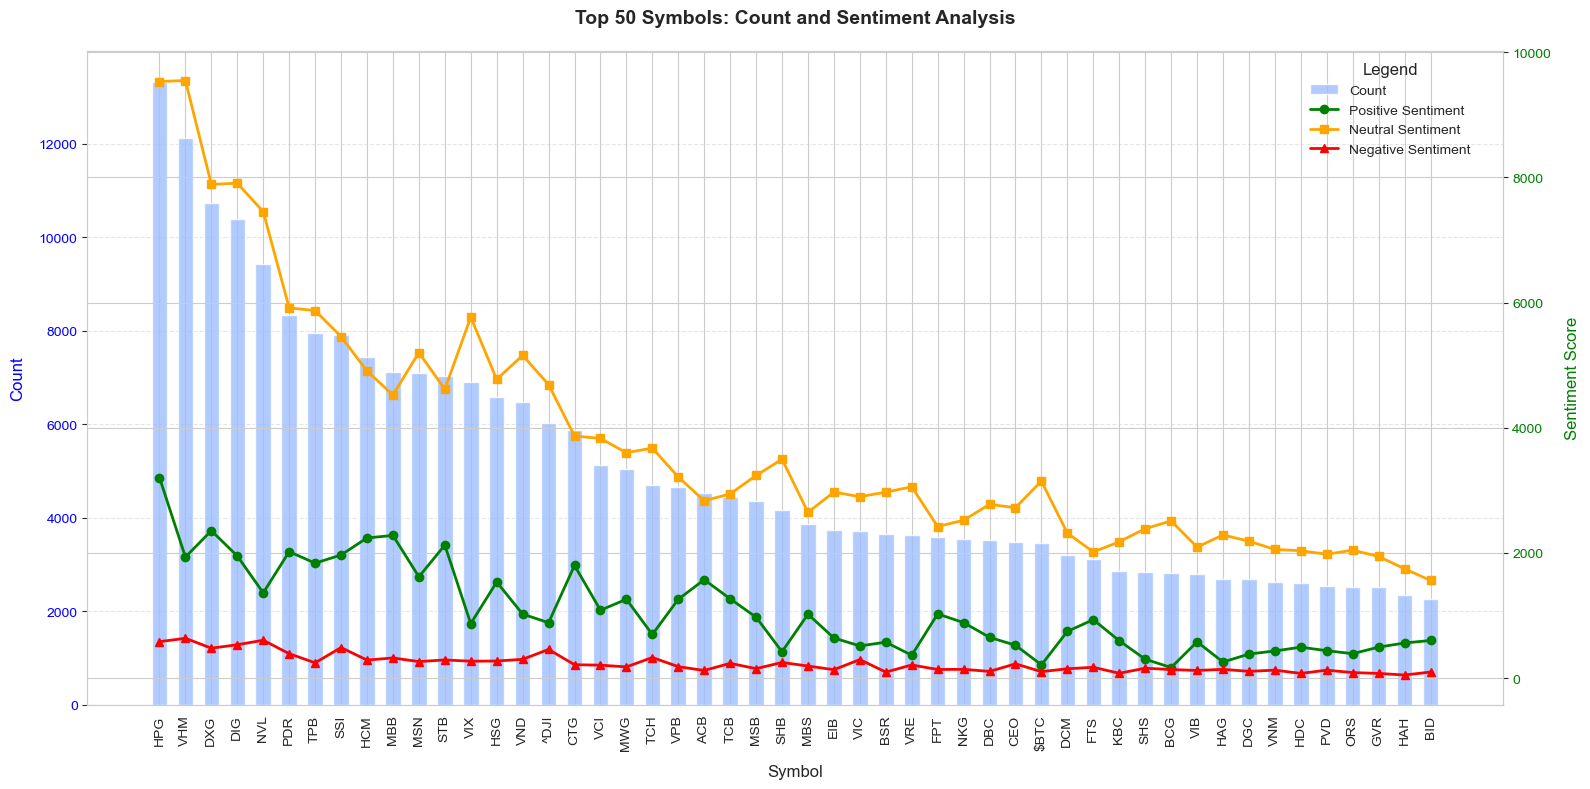
\includegraphics[width=1\linewidth]{images/plot-2.13-line_column_chart_combined.png}
    \vspace{-2em}
    \caption{Top 50 mã cổ phiếu, và quan điểm của người dùng}
    \label{fig:2.11}
\end{figure}

Từ biểu đồ trên ta biểu thị phần trăm tiêu cực và tích cực của 10 mã chứng khoán trên theo thứ tự từ trên xuống dưới.
\vspace{-0.5em}
\begin{figure}[H]
    \centering
    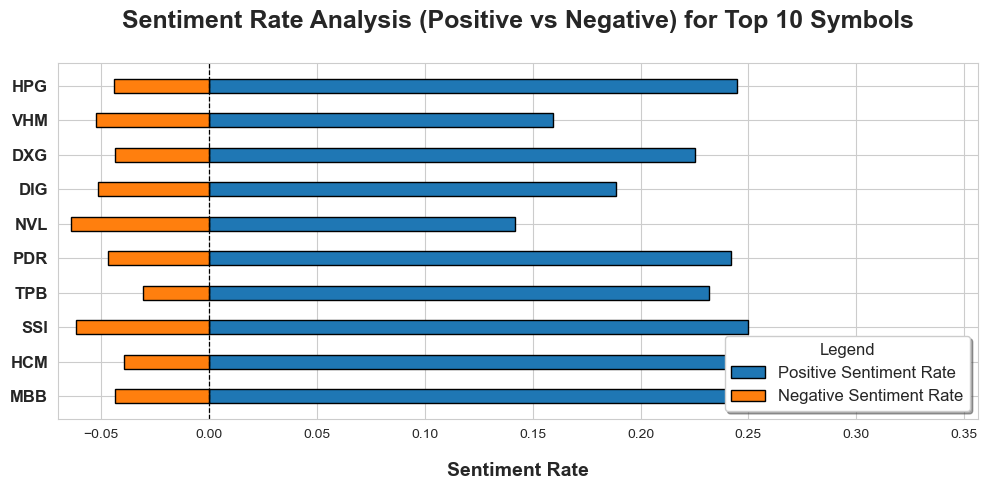
\includegraphics[width=0.95\linewidth]{images/plot-2.25-plot-bar_chart.png}
    \vspace{-1em}
    \caption{Tỉ lệ quan điểm người dùng của 10 mã có lượt đề cập nhiều nhất }
    \label{fig:2.12}
\end{figure}

\textbf{Nhận xét:}\\

Từ 2 plot trên ta thấy rằng:
\begin{itemize}
    \item Các mã được nhắc đến đều là những mã có nhiều giao dịch, và đa số là những công ty dẫn đầu ngành tương ứng, từ ngành Thép, cho tới Bất động sản, Ngân hàng, Chứng khoán. Nhìn chung là có độ phân bố Tích cực cao hơn nhiều so với Tiêu cực, có lẽ do dữ liệu được lấy trong khoảng thời gian biến động chưa đủ mạnh.
    \item \textbf{HPG, VHM, DXG} là các mã được chú ý nhiều nhất, với nhận định chủ yếu là Trung lập và Tích cực. Đây cũng chính là 3 mã có thanh khoản rất lớn trên thị trường.
\end{itemize}

\subsection{So sánh số bài đăng đề cập đến của các mã theo ngày}
\begin{figure}[H]
    \centering
    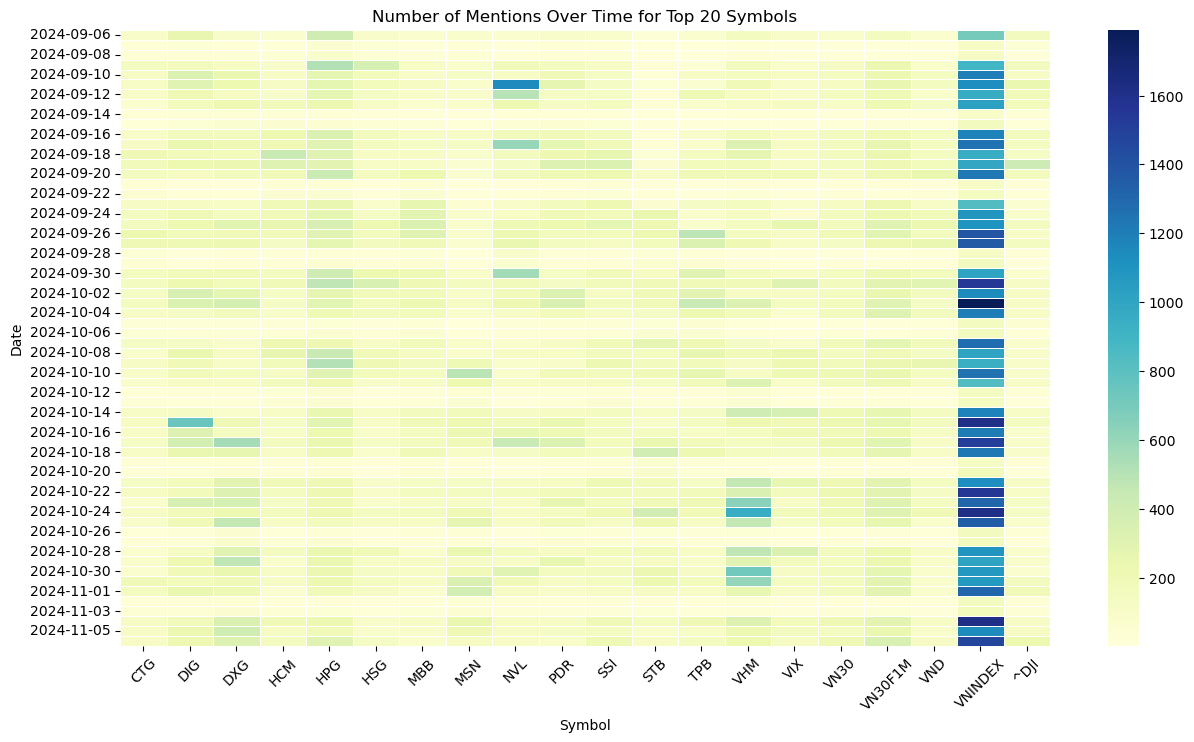
\includegraphics[width=1\linewidth]{images/plot-3.2-heatmap.png}
    \caption{Số lượt được đề cập của các mã cổ phiếu theo ngày}
    \label{fig:2.13}
\end{figure}

\textbf{Nhận xét:}
\begin{itemize}
    \item Dễ dàng nhận thấy từ hai biểu đồ trên, VNINDEX vượt trội về số lượt đề cập hàng ngày so với các mã cổ phiếu khác. 
    \item Không chỉ có vậy, số lượt đề cập đến mã cổ phiếu này trong suốt 2 tháng qua cũng rất đều đặn, cho thấy sự quan tâm rất lớn đến từ cộng đồng chứng khoán FireAnt. 
    \item Điều này hoàn toàn dễ hiểu vì VNINDEX là chỉ số đại diện cho toàn bộ thị trường chứng khoán Việt Nam. Biến động của VNINDEX có ảnh hưởng lớn đến các mã chứng khoán khác, thu hút sự chú ý mạnh mẽ từ các nhà đầu tư. 
    \item Bên cạnh VNINDEX, các mã chứng khoán đáng chú ý khác như HPG, VHM, VN30F1M, DXG và DIG cũng có số lượt đề cập ở mức khá cao. 
\end{itemize}

\subsection{Xếp hạng các mã cổ phiếu được đề cập nhiều nhất}

\begin{figure}[H]
    \centering
    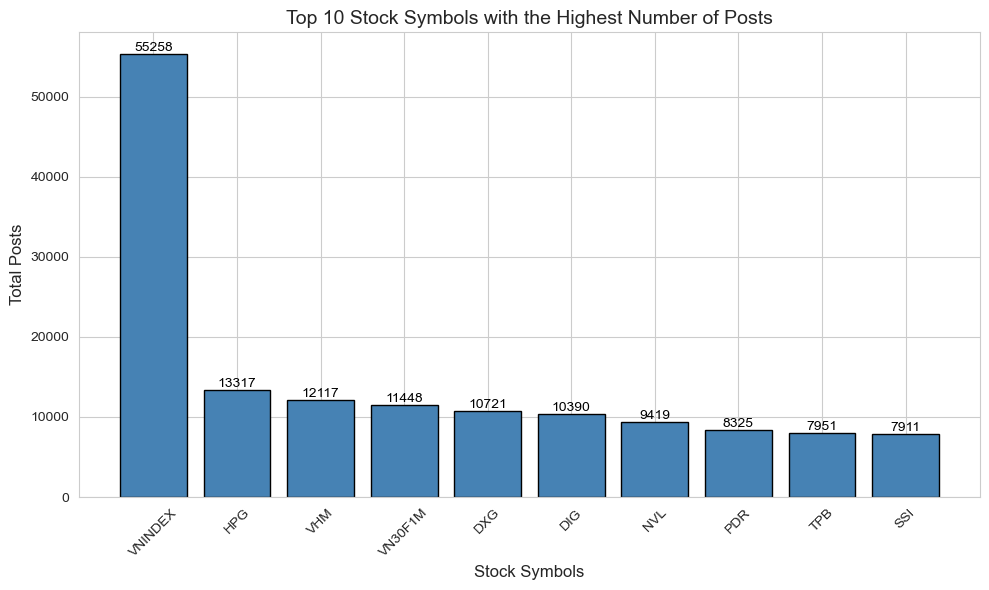
\includegraphics[width=0.9\linewidth]{images/C2_pic38.png}
    \vspace{-1em}
    \caption{Biểu đồ xếp hạng các mã cổ phiếu phổ biến nhất}
    \label{fig:2.14}
\end{figure}
\vspace{-1em}
\begin{figure}[H]
    \centering
    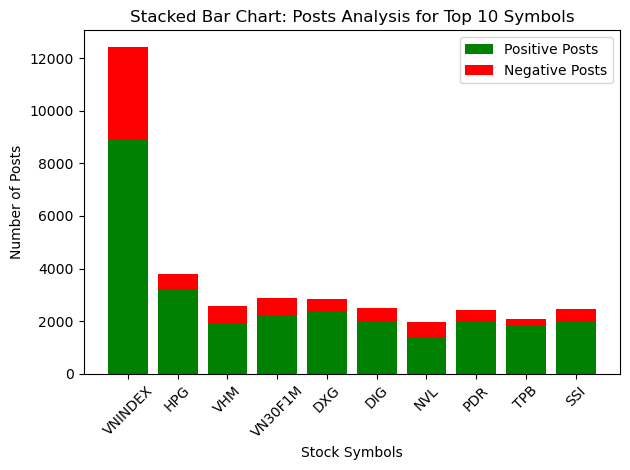
\includegraphics[width=0.65\linewidth]{images/C2_pic37.png}
    \vspace{-1em}
    \caption{Biểu đồ so sánh số bài viết tích cực và tiêu cực của các mã cổ phiếu phổ biến}
    \label{fig:2.15}
\end{figure}

\textbf{Nhận xét:}

\begin{itemize}
    \item Từ 2 biểu đồ trên, ta một lần nữa khẳng định sự phổ biến của VNINDEX, khi chỉ số này không chỉ chiếm ưu thế về số lượng bài đăng, với tổng cộng 55258 bài, mà còn cả các bài viết tich cực và tiêu cực với lần lượt 8919 và 3518 bài.
    \item Chính vì nhận được sự quan tâm lớn, VNINDEX cũng là chỉ số chịu nhiều bài viết tiêu cực cao nhất. Tỷ lệ giữa số bài viết tích cực và tiêu cực về VNINDEX chỉ là 2.5, trong khi tỷ lệ này với các mã chứng khoán khác thường trên 5.
\end{itemize}

\section{Phân tích Cộng đồng người dùng FireAnt}
\subsection{Thống kê cơ bản}
\textbf{Tổng số lượng người dùng xuất hiện trong bài đăng và phản hồi}: 24993 người.

\begin{center}
    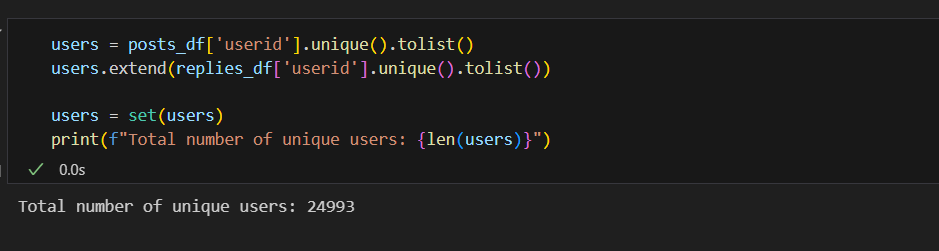
\includegraphics[width=0.75\linewidth]{images/C2_pic54.png}
\end{center}

Thoạt nhìn, con số 24.993 người dùng có các hoạt động đăng bài và phản hồi trong vòng 2 tháng có vẻ là lớn. Tuy nhiên, theo như dữ liệu công bố trên trang chủ, hiện tại FireAnt đã đạt mốc hơn 3 triệu người dùng \cite{fireant}. Do đó, số lượng người dùng tham gia hoạt động thực tế chỉ chiếm một tỷ lệ rất nhỏ so với tổng số người dùng đã đăng ký trên nền tảng. \\

Điều này thể hiện rằng phần lớn người dùng có xu hướng theo dõi thông tin hơn là tương tác. Hoạt động trên nền tảng có thể tập trung vào một nhóm người dùng tích cực, trong khi đa số còn lại thụ động. Ngoài ra, số liệu này chỉ phản ánh trong 2 tháng, có thể chưa đủ để đánh giá toàn diện mức độ tham gia trên nền tảng.\\

\textbf{Tổng số người dùng có trên 100 bài viết}: 387 người.

\textbf{Tổng số người dùng có trên 100 lượt phản hồi}: 87 người.

\begin{center}
    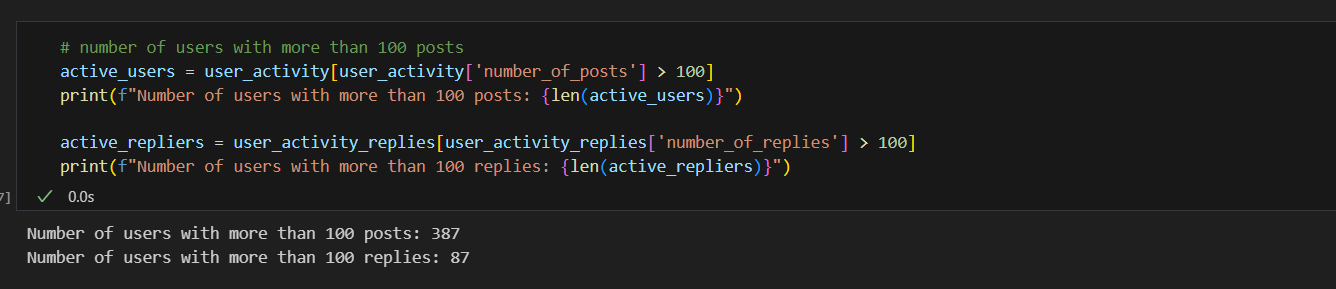
\includegraphics[width=0.95\linewidth]{images/C2_pic53.png}
\end{center}

Điều này phản ánh rằng nội dung chủ yếu được tạo bởi một nhóm nhỏ người dùng tích cực, ngoài ra cũng khá thú vị khi số người bình luận lại ít hơn số người đăng bài.\\

\textbf{Thống kê số lượng người dùng đăng bài mỗi ngày}
\vspace{-1em}
\begin{figure}[H]
    \centering
    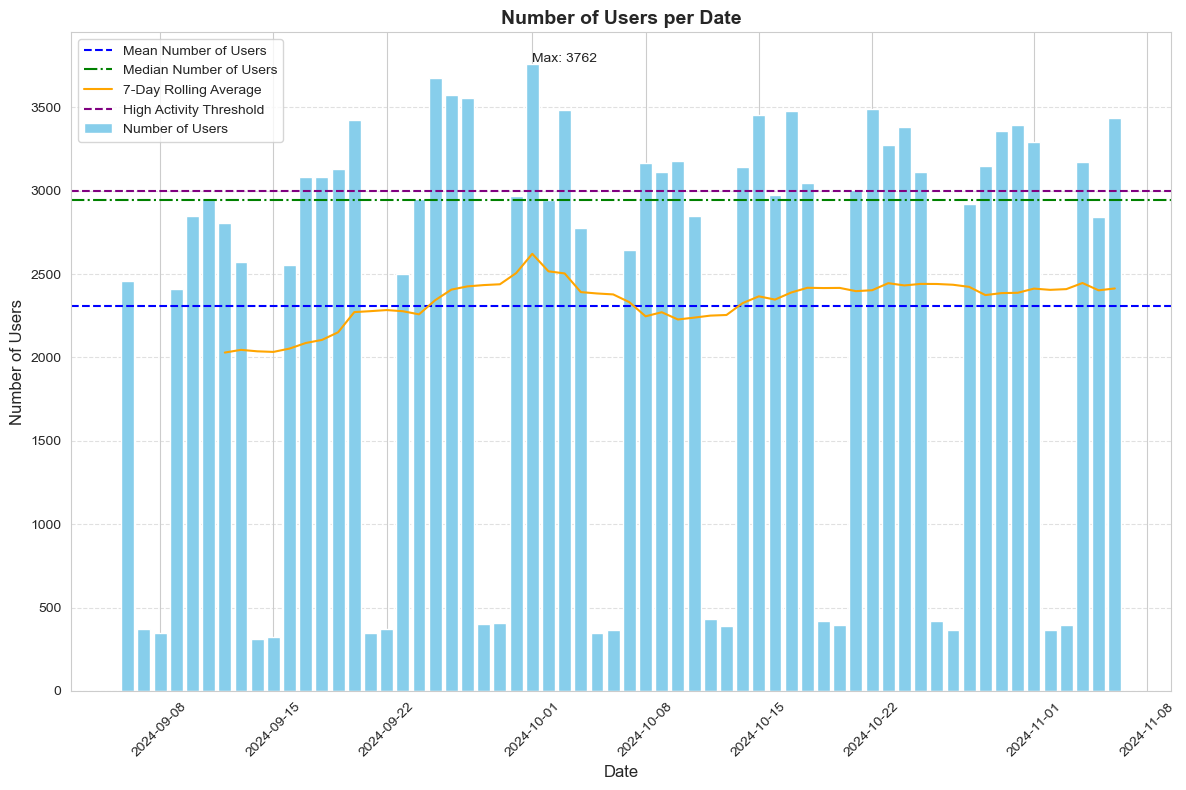
\includegraphics[width=0.75\linewidth]{images/C2_pic49.png}
    \vspace{-1.2em}
    \caption{Biểu đồ Thống kê lượng người dùng đăng bài mỗi ngày}
    \label{fig:2.16}
\end{figure}

Dễ thấy, số lượng người hoạt động trên diễn đàn FireAnt có sự thay đổi theo chu kỳ, với 5 ngày cao điểm và 2 ngày thấp điểm. Tương quan lớn với biểu đồ số lượng bài viết/phản hồi (\ref{fig:2.1}), (\ref{fig:2.8}).\\

\textbf{Thống kê số lượng người tham gia phản hồi theo ngày}

\begin{figure}[H]
    \centering
    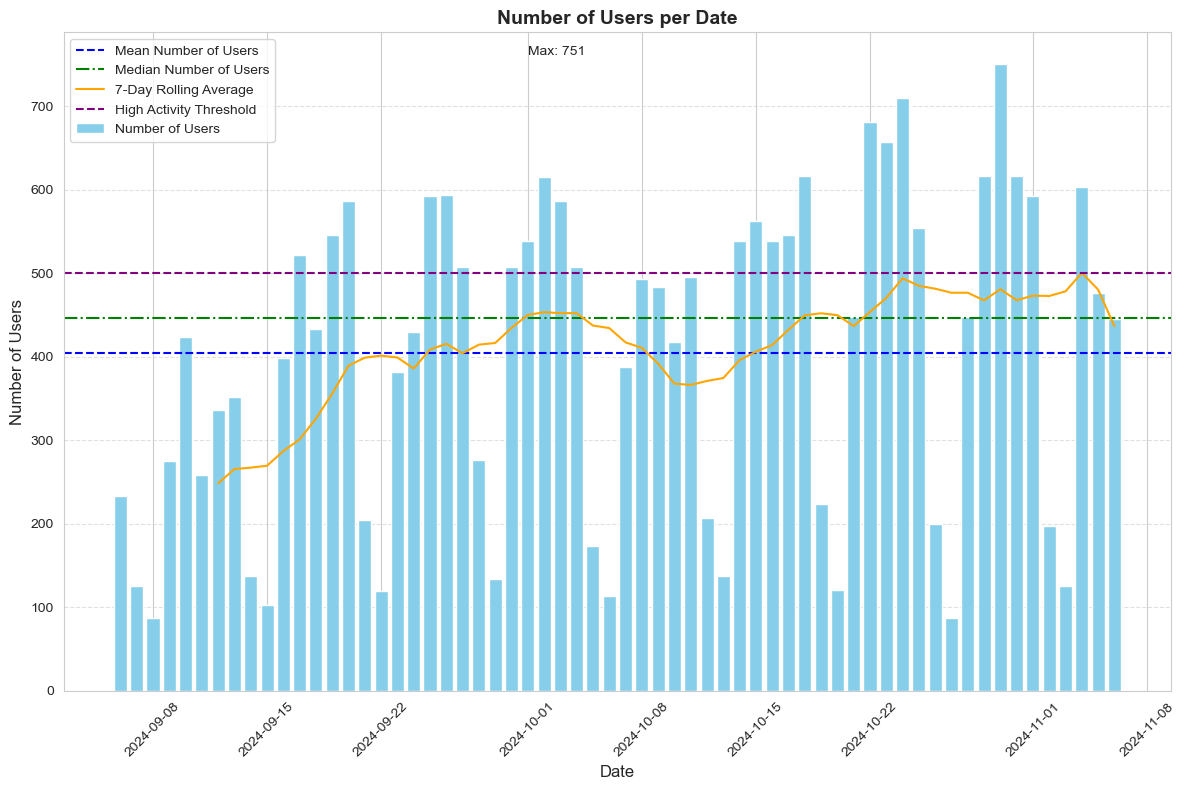
\includegraphics[width = 0.75\linewidth]{images/C2_pic51.png}
    \vspace{-1.2em}
    \caption{Số lượng người tham gia phản hồi theo ngày}
    \label{fig:2.17}
\end{figure}

Tương tự với số người đăng bài, số người phản hồi cũng thay đổi theo chu kỳ, với 5 ngày cao điểm và giảm mạnh vào hai ngày cuối tuần (Thứ Bảy và Chủ Nhật). Tuy nhiên, số người tham gia phản hồi nhìn chung vẫn thấp hơn đáng kể so với số người đăng bài.\\

\textbf{Hệ số tương quan giữa số người dùng và số bài đăng}
\begin{center}
     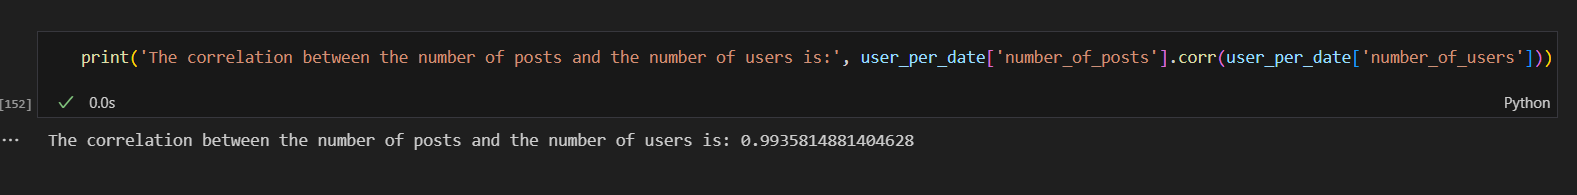
\includegraphics[width=1\linewidth]{images/C2_pic52.png}
\end{center}
\vspace{-1em}
\begin{figure}[H]
    \centering
    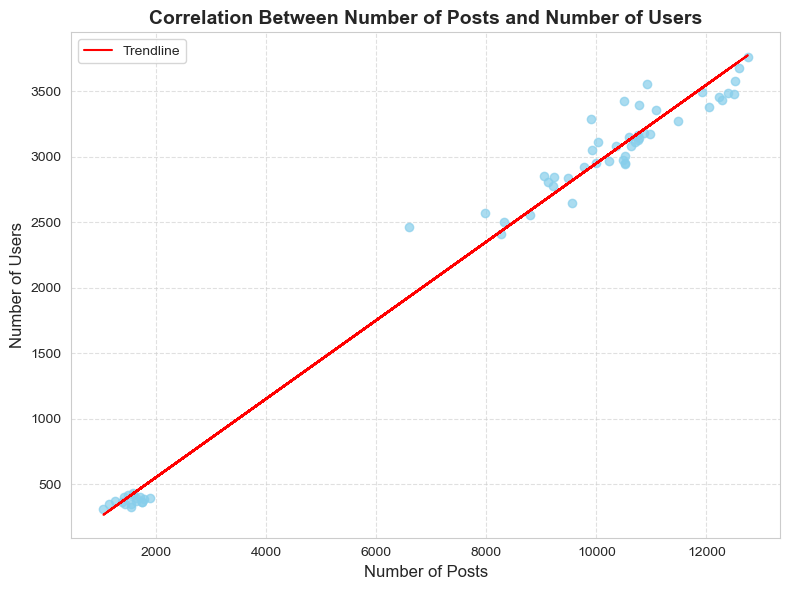
\includegraphics[width=0.55\linewidth]{images/C2_pic50.png}
    \vspace{-1em}
    \caption{Tương quan giữa Số lượng bài viết và Số người dùng}
\end{figure}

Ta thấy số lượng bài đăng có mối liên hệ chặt chẽ với số lượng người đăng bài, thể hiện qua hệ số tương quan lên tới 0.9936. Đây là điều hoàn toàn hiển nhiên, vì số lượng bài đăng tăng đồng nghĩa với việc có nhiều người tham gia hoạt động hơn.\\

\textbf{Thống kê Số phản hồi trong mỗi bài đăng}

\begin{figure}[H]
    \centering
    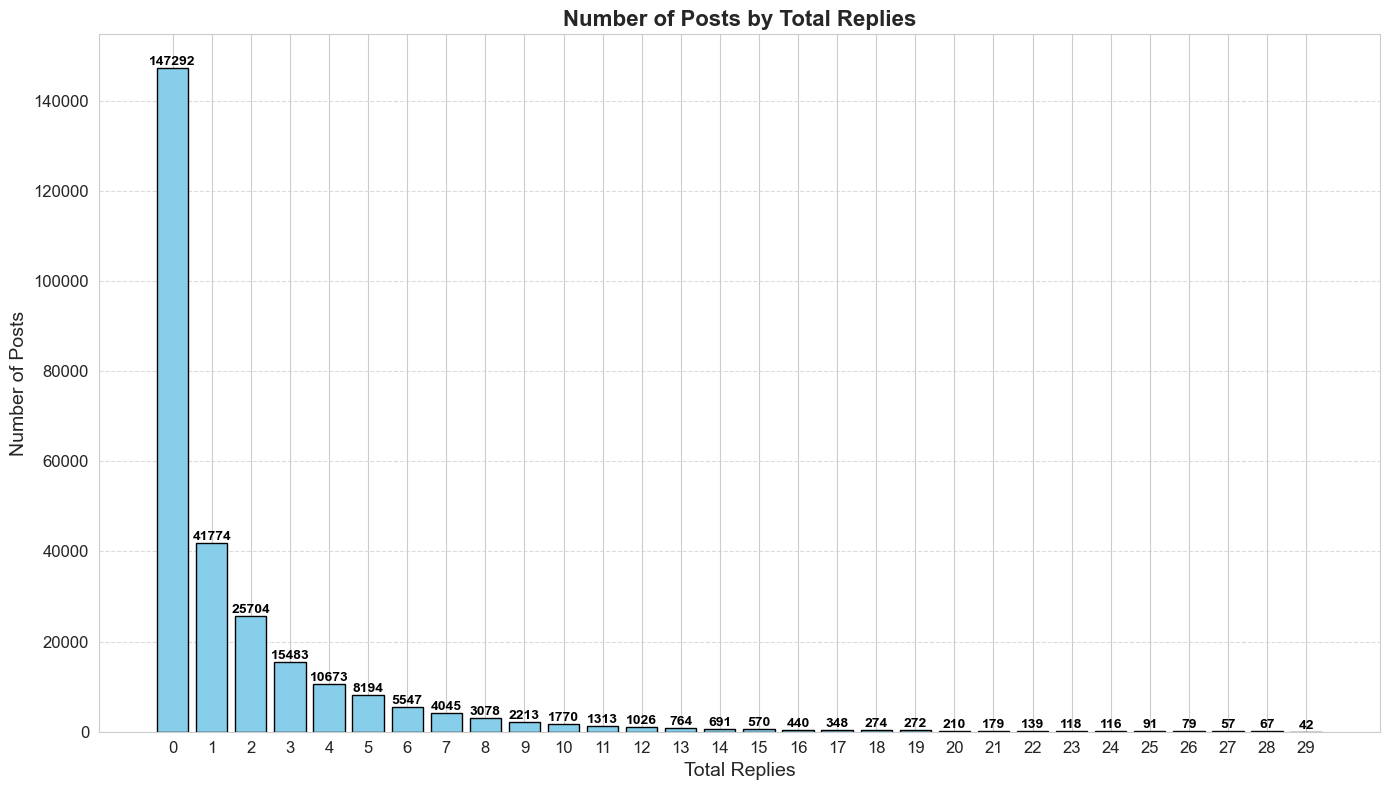
\includegraphics[width = 1\linewidth]{images/C2_pic57.png}
    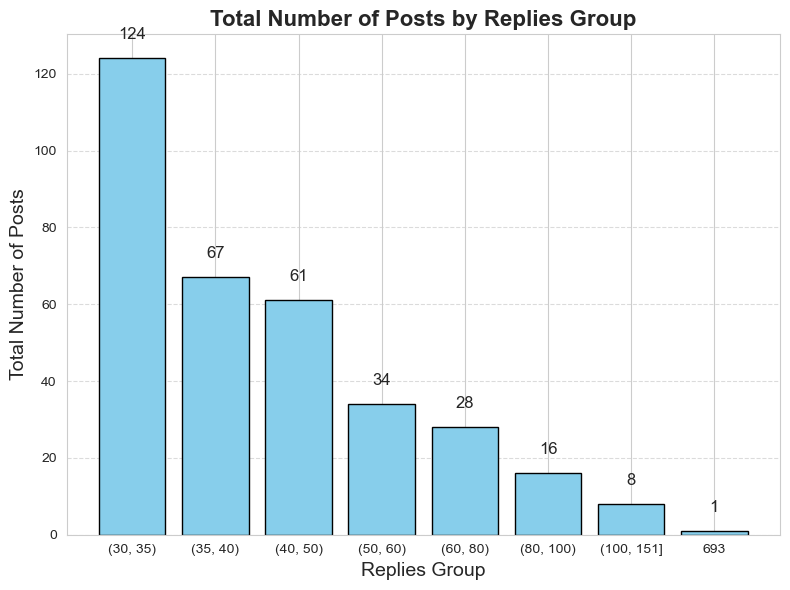
\includegraphics[width = 0.7\linewidth]{images/C2_pic56.png}
    \vspace{-1em}
    \caption{Thống kê Số phản hồi trong mỗi bài đăng}
\end{figure}

Ta thấy phần lớn các bài đăng trên điễn đần FireAnt đều không có hoặc có rất ít phản hồi. Cụ thể trong tổng số hơn 270 nghìn bài viết mà ta đã cào được, có đến $147.292\ (\approx54\%)$ bài viết là không có phản hồi. Số bài có từ 5 phản hồi trở xuống chiếm đến 91.26\%. Điều này cho thấy mức độ tương tác của người dùng là tương đối thấp.\\

Một số bài viết đạt từ 50 lượt phản hồi trở lên, hầu hết là những bài viết ``tóm tắt diễn biến thị trường trong ngày'', thu hút được nhiều người dùng vào bình luận và trao đổi.\\

Tuy vậy vẫn có một trường hợp ngoại lệ xảy ra, vào ngày 26/9/2024, người dùng \textbf{Doan Nhan} đã đăng \href{https://fireant.vn/dashboard/content/posts/28340183/replies}{một bài viết} chỉ với 5 chữ ``Thức dậy đi chú Đạt'' nhưng có đến 693 lượt phản hồi. Thực ra hầu hết đoạn phản hồi ở đây là cuộc tranh cãi qua lại giữa người này và một người dùng khác trong 5 tuần, còn ``chú Đạt'' ở đây là Chủ tịch của công ty Phát Đạt (PDR).

\newpage
\subsection{Thống kê các hoạt động nổi bật của người dùng}
\subsubsection{Xếp hạng người dùng có số bài đăng lớn nhất}

\begin{figure}[H]
    \centering
    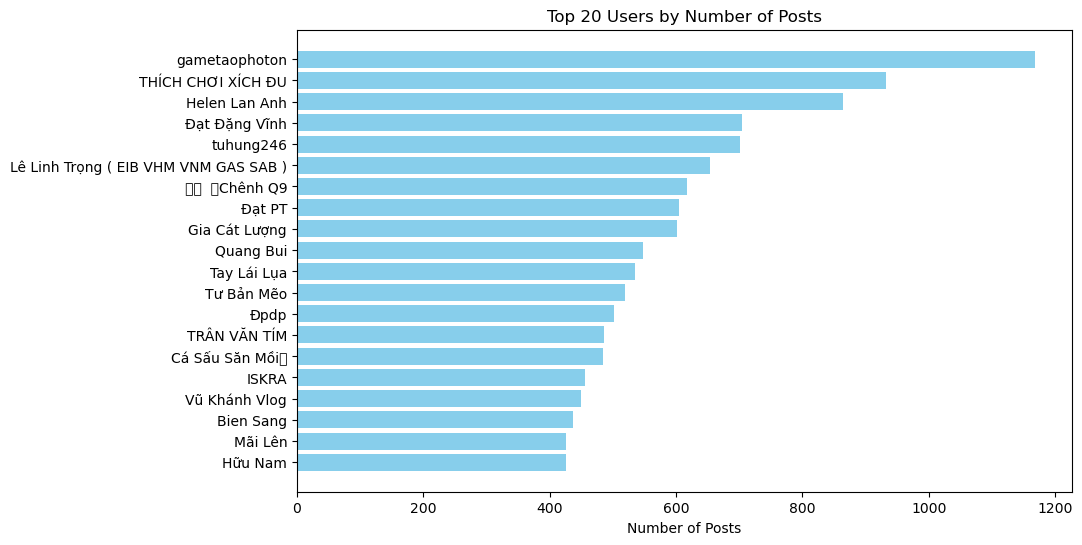
\includegraphics[width = 0.85\linewidth]{images/C2_pic27.png}
    \vspace{-1em}
    \caption{Thống kê Top 20 người dùng đăng bài nhiều nhất}
    \label{fig:2.18}
\end{figure}

Dễ thấy, \texttt{gam**ton}, \texttt{Thí**đu}, hay \texttt{Hel**Anh} là những người dùng có hoạt động tích cực nhất, nổi trội hơn hẳn so với những người còn lại trong danh sách. Tuy vậy, các tài khoản này thường xuyên đăng tải nội dung với tần suất rất cao, chủ yếu là các bài viết có tính chất spam hoặc chia sẻ những thông tin lặp đi lặp lại. Những hành vi này cho thấy hoạt động của các tài khoản trên không thực sự mang lại giá trị lớn cho cộng đồng, mà chủ yếu chỉ để tăng sự hiện diện cá nhân hoặc phục vụ mục đích riêng.

\subsubsection{Xếp hạng người dùng có số lượt phản hồi và lượt thích cao nhất}
\begin{figure}[H]
    \centering
    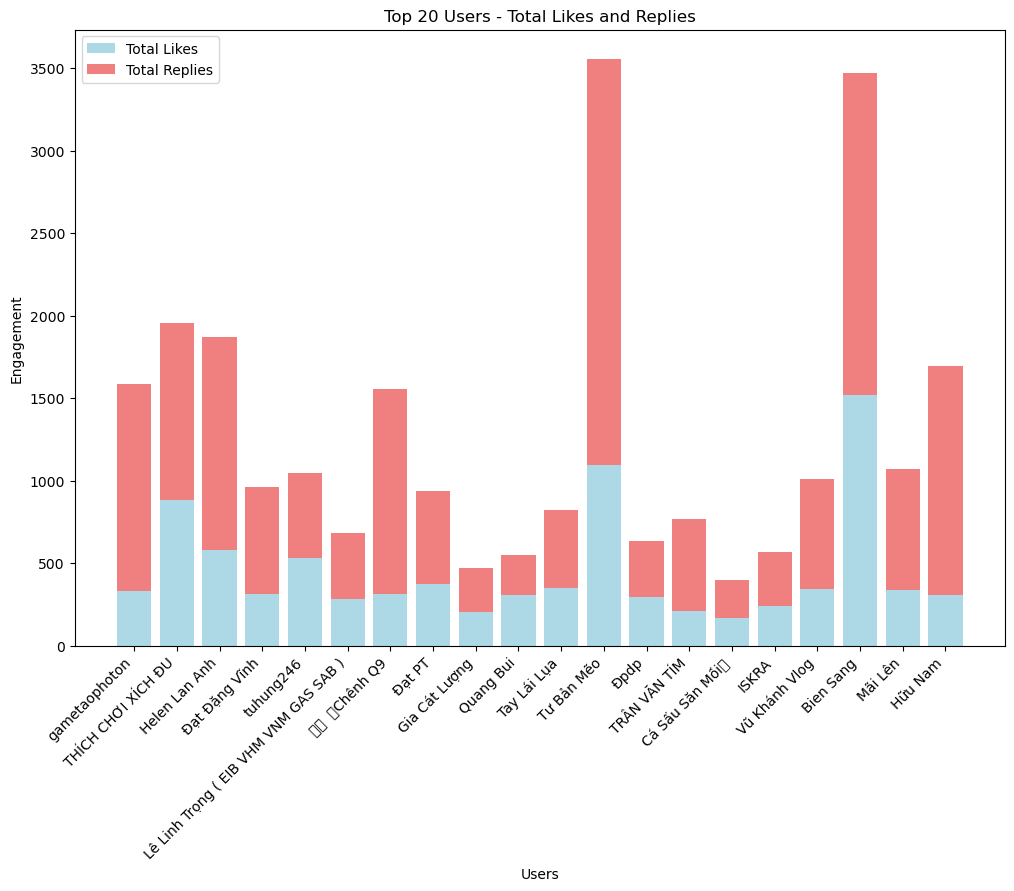
\includegraphics[width = 0.75\linewidth]{images/C2_pic28.png}
    \vspace{-1em}
    \caption{Thống kê Top 20 người dùng có nhiều lượt thích và bình luận nhất}
    \label{fig:2.19}
\end{figure}

Ở biểu đồ này, ta có thể thấy không phải \texttt{gam**ton} hay \texttt{Hel**Anh} là những người đứng đầu về tầm ảnh hưởng, mà chính \texttt{Tư**Mẽo} và \texttt{Biên Sang} mới thực sự nổi bật. Mặc dù số bài đăng của hai người dùng này chưa bằng một nửa so với \texttt{gam**ton}, nhưng tổng số lượt tương tác mà họ nhận được lại gấp đôi.\\

Điều này phần lớn là do các bài viết của \texttt{Tư**Mẽo} và \texttt{Biên Sang} thường mang tính phân tích sâu sắc về thị trường chứng khoán và chia sẻ kinh nghiệm đầu tư thực tiễn (\texttt{Tư**Mẽo} đề cập tới 46 mã cổ phiếu trong các bài đăng của mình).

\subsubsection{Xếp hạng người dùng tích cực phản hồi các bài viết nhất}
\begin{figure}[H]
    \centering
    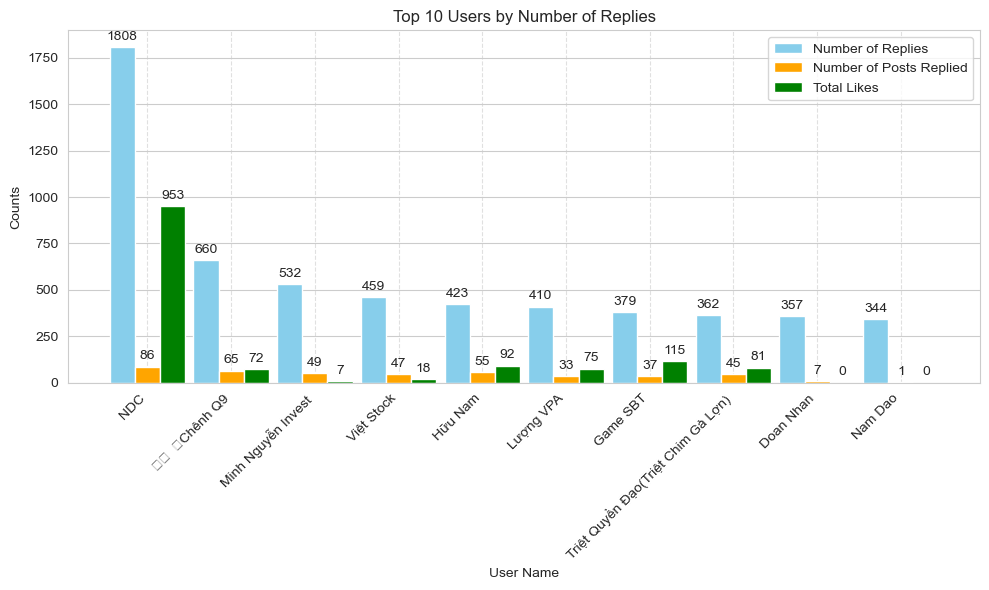
\includegraphics[width = 0.75\linewidth]{images/C2_pic47.png}
    \vspace{-1em}
    \caption{Thống kê Top 10 người dùng bình luận nhiều nhất}
    \label{fig:2.20}
\end{figure}

Ta thấy người dùng \texttt{NDC} vượt trội cả về số bài phản hồi và tổng lượt thích. Mặc dù chỉ bình luận cho 86 bài viết, nhưng đã viết hơn 1800 bài và nhận được 953 lượt thích, điều này cho thấy mức độ tương tác rất cao với cộng đồng. Có nhiều người dùng chỉ bình luận, chứ không thường xuyên đăng bài hay thích một bài.

\subsubsection{Xếp hạng người dùng có độ chính xác quan điểm cao nhất}

Ta sẽ đặt ra một phép đo, thể hiện tần suất bài đăng của một người dùng cụ thể ``dự đoán đúng'' giá cổ phiếu trong phiên giao dịch tiếp theo. Ví dụ, khi bài đăng thể hiện quan điểm Tiêu cực, và giá cổ phiếu đi xuống; hay khi bài viết Tích cực và giá cổ phiếu đi lên; lúc đó bài đăng này được coi là ``dự đoán đúng''.

\[
\text{Độ chính xác} = \frac{\text{Số bài dự đoán đúng}}{\text{Tổng số bài có Quan điểm}}
\]

\begin{center}
    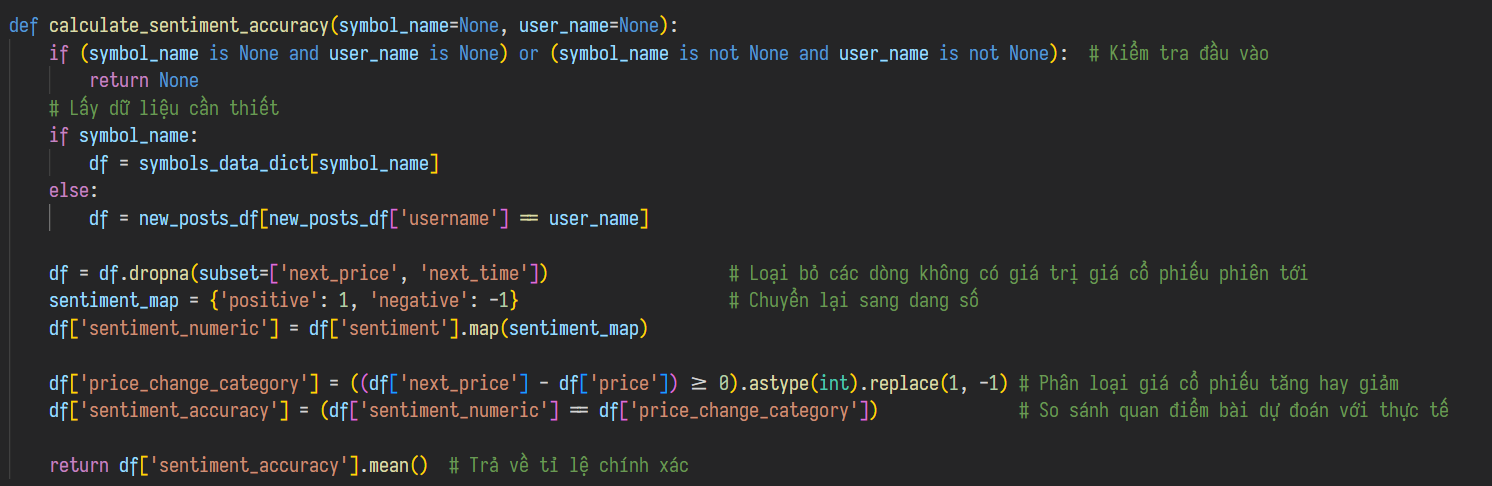
\includegraphics[width=1\linewidth]{images/code-2.20-sentimentacc.png}
\end{center}

\begin{figure}[H]
    \centering
    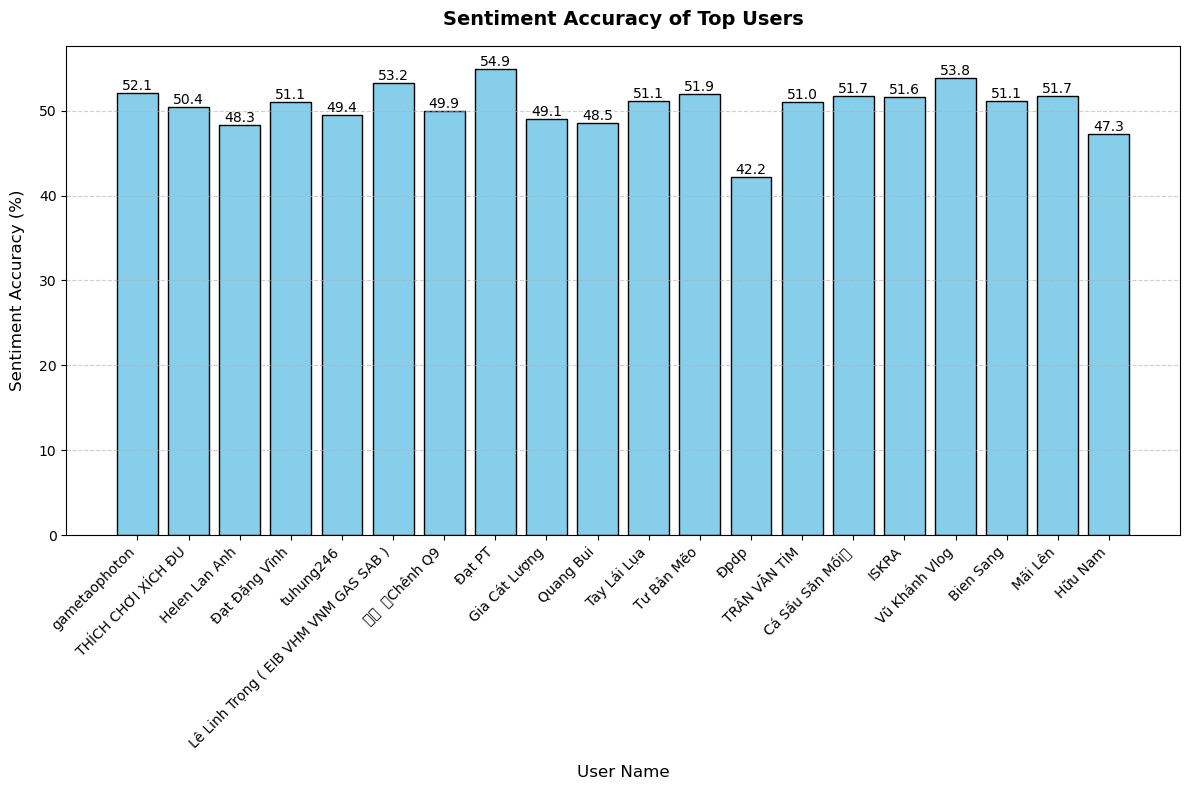
\includegraphics[width = 0.75\linewidth]{images/C2_pic19.png}
    \caption{So sánh Độ chính xác quan điểm của người dùng hay đăng bài}
    \label{fig:2.21}
\end{figure}

Ta nhận thấy độ chính xác của các người đăng bài nhiều nhất đều không cao. Người dùng đứng đầu chỉ có độ chính xác là 54.9\%. Nhìn chung các người dùng khác cũng chỉ có độ chính xác loanh quanh 50\%, do đó ta có thể kết luận, việc dựa trên các bài viết tiêu cực và tích cực của người dùng hay đăng bài để đoán giá là khó khả thi.

\subsubsection{Thống kê những người dùng phổ biến nhất theo từng khung giờ}
\vspace{-1em}
\begin{figure}[H]
    \centering
    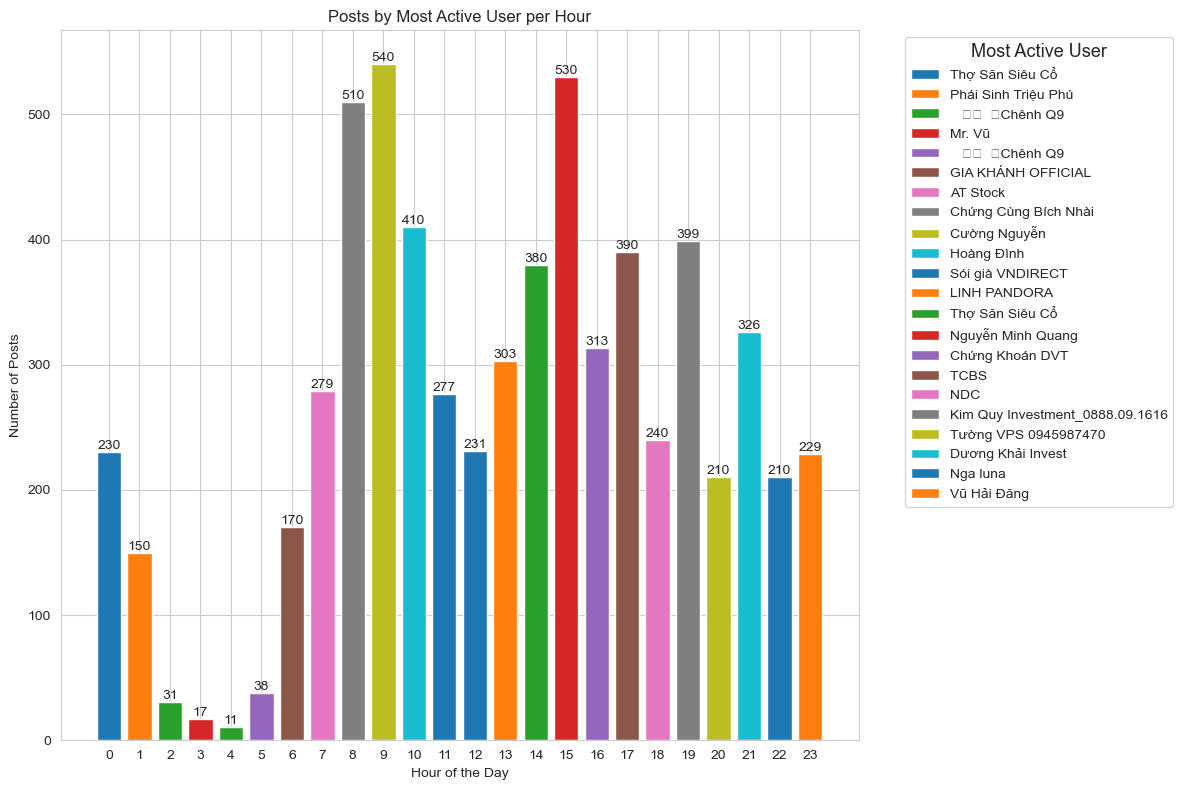
\includegraphics[width = 1\linewidth]{images/C2_pic55.png}
    \vspace{-2em}
    \caption{Thống kê những người dùng phổ biến nhất theo từng khung giờ}
    \label{fig:2.22}
\end{figure}
\vspace{-0.5em}
Ở đây, ta có thể thấy một số cái tên quen thuộc đã xuất hiện từ trước. Đặc biệt, \texttt{Chê**Q9} nổi bật với việc đăng bài vào những khung giờ rất muộn như 2h và 4h sáng.

\subsection{Phân tích Văn hóa ứng xử của người dùng}
Sự văn minh và thân thiện giữa người dùng và người sáng tạo nội dung là yếu tố quan trọng quyết định sự phát triển bền vững của một cộng đồng. Vì vậy, chúng ta sẽ cùng phân tích xem FireAnt có thực sự là một môi trường giao tiếp tích cực và xây dựng, nơi các cuộc thảo luận diễn ra trong không khí tôn trọng và xây dựng, hay liệu vẫn tồn tại các vấn đề liên quan đến hành vi không phù hợp, như việc sử dụng ngôn từ tục tĩu hoặc thiếu văn minh.\\

Ta sẽ sử dụng nguồn từ chửi tục trong file \texttt{Vietnamese\_cursed\_words.txt}, biến đổi từ file gốc \cite{vnoffensive}. Trước hết ta cần phải lọc dấu câu, biến toàn bộ ký tự trong cột \texttt{originalContent} thành chữ thường. Sau đó chỉ cần làm một hàm đếm số lượng từ chửi tục:

\begin{center}
    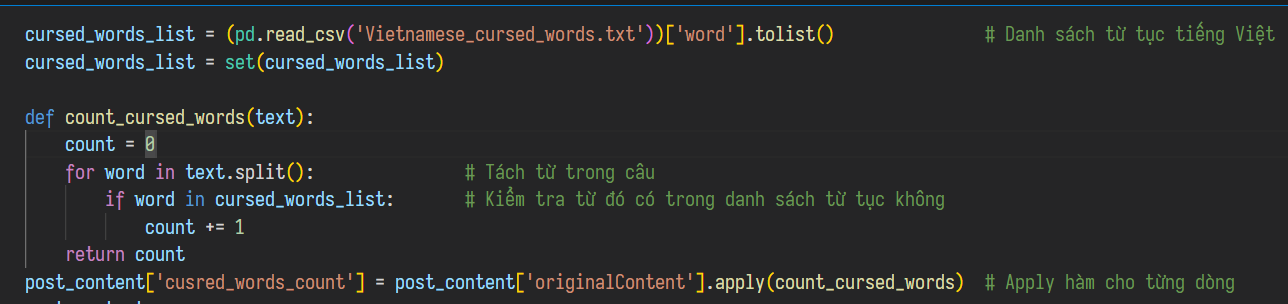
\includegraphics[width=1\linewidth]{images/code-2.24.png}
\end{center}

\subsubsection{Số lượng bài đăng dựa trên số lượng các từ chửi tục}
  \begin{figure}[H]
      \centering
      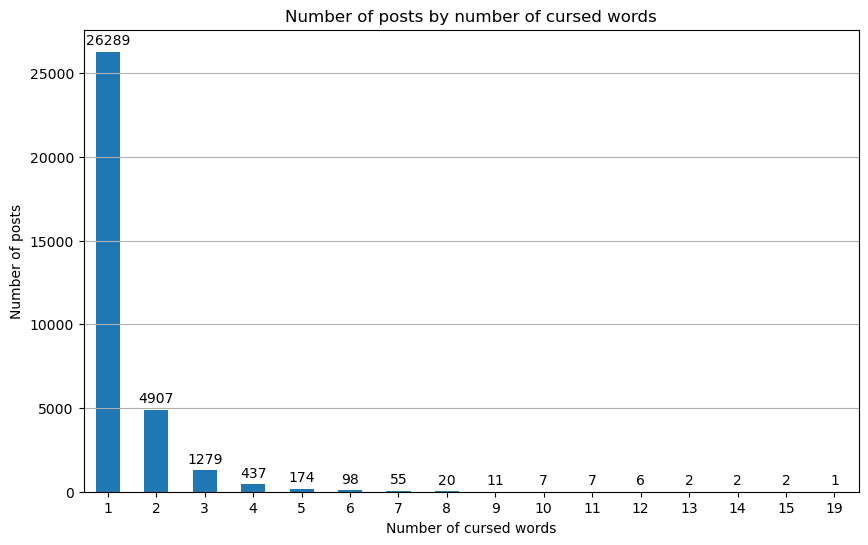
\includegraphics[width=0.8\linewidth]{images/C2_pic39.png}
      \caption{Số lượng bài đăng dựa trên số lượng các từ chửi tục}
      \vspace{-1em}
      \label{fig:2.23}
  \end{figure}
    
\textbf{Nhận xét:}
\begin{itemize}
    \item Ta thấy trong các bài đăng kém văn minh, phần lớn chỉ có 1 từ chửi thề, số từ chửi thề càng lớn, số bài đăng càng giảm.
    \item Số từ chửi tục lớn nhất có trong 1 bài đăng là 19, cho thấy mức độ cay cú của người viết bài.
\end{itemize}

\subsubsection{Tỉ lệ Quan điểm của những bài có chửi tục}
\begin{figure}[H]
    \centering
    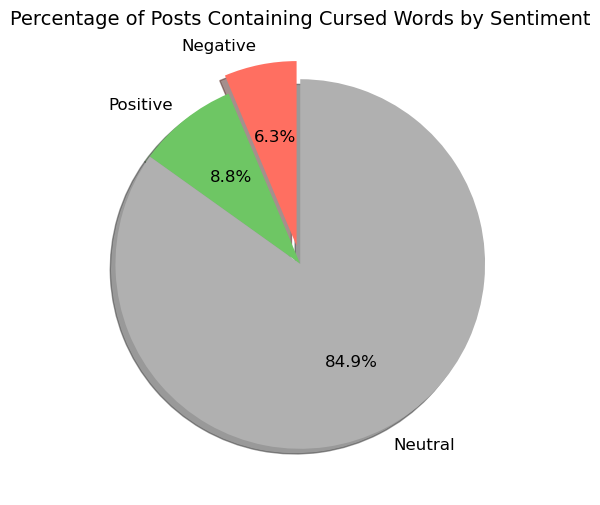
\includegraphics[width=0.55\linewidth]{images/C2_pic41.png}
    \vspace{-1em}
      \caption{Tỉ lệ Quan điểm của những bài có chửi tục}
      \label{fig:2.24}
\end{figure}
Dễ thấy đa phần các bài viết, đều là các bài viết trung lập. Điều này đa phần do người dùng ở diễn đần FireAnt quên không phân định quan điểm bài viết trước khi đăng. Điều khá thú vị là số lượng bài Tích cực chửi tục lại nhiều hơn Tiêu cực, điều này chứng tỏ rằng, người dùng không chỉ mỗi chửi tục khi thể hiện quan điểm Tiêu cực.

\subsubsection{Xếp hạng các người dùng kém văn minh nhất}

\begin{figure}[H]
    \centering
    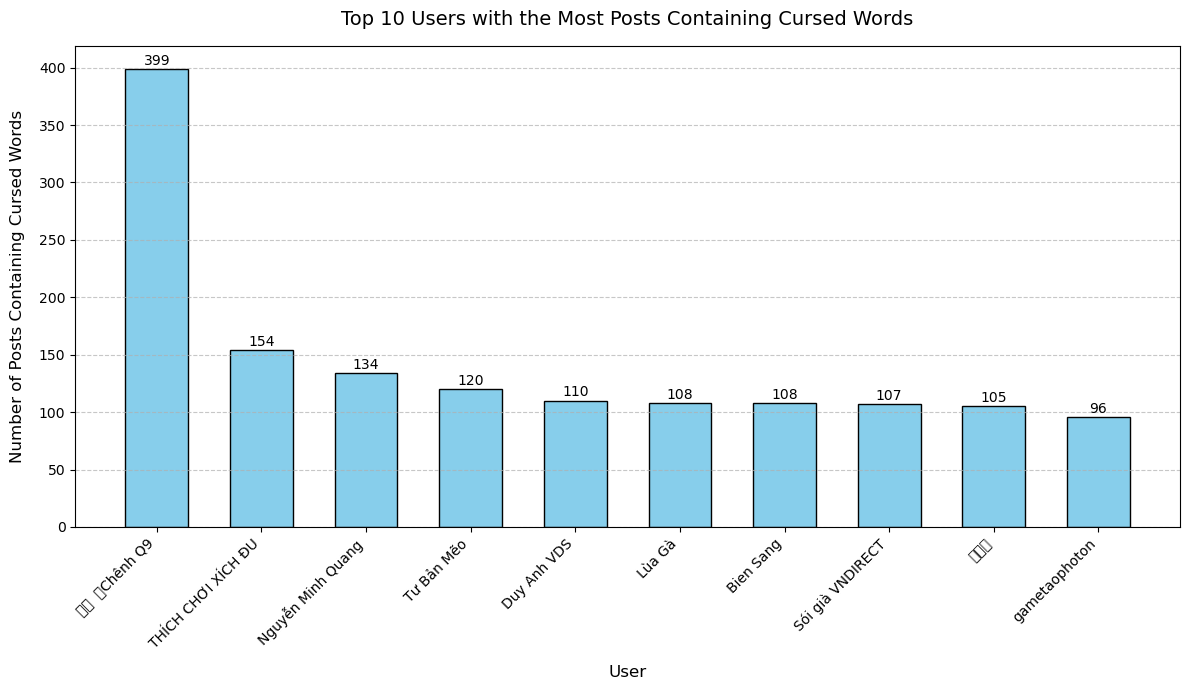
\includegraphics[width=0.85\linewidth]{images/C2_pic35.png}
    \caption{Xếp hạng những người dùng có bài viết chửi tục nhiều}
    \label{fig:2.25}
\end{figure}

\begin{figure}[H]
    \centering
    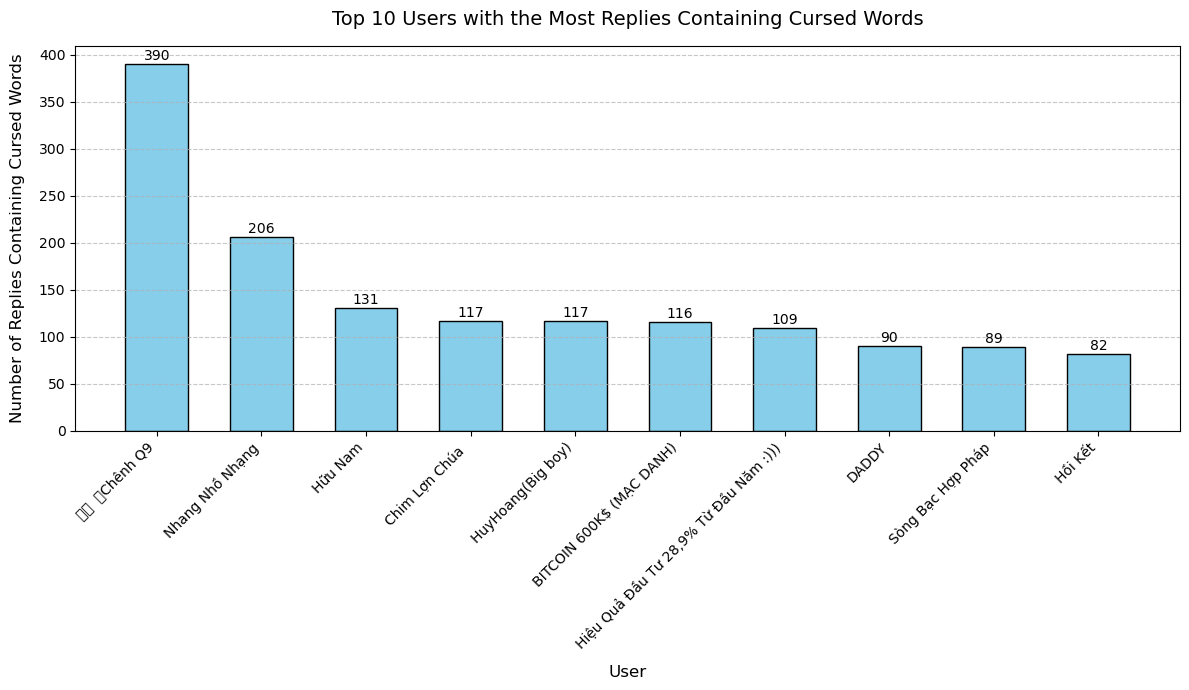
\includegraphics[width=0.85\linewidth]{images/C2_pic36.png}
    \caption{Xếp hạng những người dùng có bình luận chửi tục nhiều}
    \label{fig:2.26}
\end{figure}

Người dùng \texttt{Chê**Q9} nổi bật nhất với 399 bài viết và 390 bình luận chứa các từ ngữ chửi tục. Mặc dù đây là những người có số lượng bài viết ...vô văn hoá nhiều nhất, nhưng họ cũng là những người có số lượng lượt thích và bình luận cao. Có thể những nội dung tiêu cực, hoặc sử dụng ngôn ngữ mạnh thường thu hút sự chú ý và tương tác cao từ cộng đồng. 

\subsubsection{So sánh tỷ lệ các bài đăng văn minh và các bài đăng kém văn minh}
\vspace{-1em}
\begin{figure}[H]
  \begin{subfigure}{.47\textwidth}
  \centering
    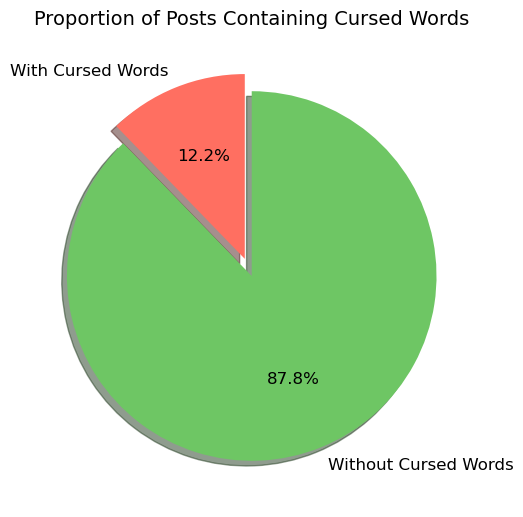
\includegraphics[width=1\linewidth]{images/C2_pic42.png}
    \caption{Tỉ lệ Bài viết}
  \end{subfigure}
  \begin{subfigure}{.53\textwidth}
  \centering
    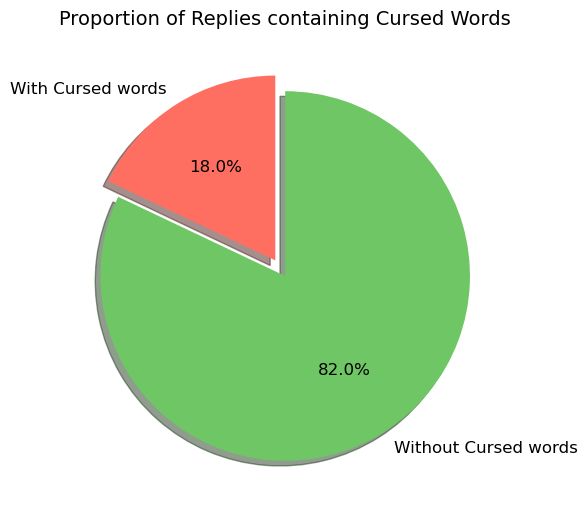
\includegraphics[width=1\linewidth]{images/C2_pic40.png}
    \caption{Tỉ lệ Bình luận}
  \end{subfigure}%
  \caption{Tỉ lệ chửi tục trong bài viết/bình luận}
  \label{fig:2.27}
\end{figure}
\vspace{-1em}
\textbf{Nhận xét:}

\begin{itemize}
    \item Từ hai biểu đồ so sánh trên, ta có thể ghi nhận một dấu hiệu tích cực về mức độ lịch sự trong các bài viết của người dùng.
    \item Cụ thể, 88\% các bài đăng gốc và 82\% các bài phản hồi là những bài viết lịch sự, không chứa từ ngữ chửi tục.
    \item Điều này cho thấy phần lớn người dùng vẫn giữ được thái độ văn minh trong giao tiếp trên mạng, đặc biệt trong các bài đăng gốc.
\end{itemize}
